%%%%%%%%%%%%%%%%%%%%%%%%%%%%%%%%%%%%%%%%%%%%%%%%%%%%%%%%%%%%%%%%%%%%%%%%%%%%%%%%%%%%%
% PACOTES                                                                           %
%%%%%%%%%%%%%%%%%%%%%%%%%%%%%%%%%%%%%%%%%%%%%%%%%%%%%%%%%%%%%%%%%%%%%%%%%%%%%%%%%%%%%
\documentclass[a4paper,11pt]{article}

%-----------------------------------------------------------------------------------%
% LAYOUT DA PÁGINA                                                                  %
%-----------------------------------------------------------------------------------%
\usepackage[top=2.25cm, bottom=2.25cm, left=2.25cm, right=2.25cm]{geometry}
%\usepackage{fancyhdr} % Permite controlar como são exibidos os cabeçalhos

%-----------------------------------------------------------------------------------%
% FORMATAÇÃO DO TEXTO                                                               %
%-----------------------------------------------------------------------------------%
%\usepackage{setspace} % Permite definir o espaçamento entre linhas

%-----------------------------------------------------------------------------------%
% PACOTES DE IMAGENS                                                                %
%-----------------------------------------------------------------------------------%
\usepackage[pdftex]{graphicx}
\pdfsuppresswarningpagegroup=1 % A warning issued when several PDF images are
% imported in the same page. Mostly harmless, can be almost always supressed.
%\usepackage[pstarrows]{pict2e} % Amplia as funcionalidades do ambiente picture
\usepackage{tikz}
\usetikzlibrary{shapes, arrows, arrows.meta}

%-----------------------------------------------------------------------------------%
% PACOTES DE TABELAS                                                                %
%-----------------------------------------------------------------------------------%
\usepackage{array} % Facilita a formatação de tabelas
%\usepackage{multirow} % Permite criar células que ocupam várias linhas em uma tabela
\usepackage{longtable} % Permite criar tabelas que quebram de página

%-----------------------------------------------------------------------------------%
% PACOTES MATEMÁTICOS DE BASE                                                       %
%-----------------------------------------------------------------------------------%
\usepackage{amsfonts,amstext,amscd,bezier,amsthm,amssymb}
\usepackage[centertags]{amsmath}

%-----------------------------------------------------------------------------------%
% PACOTES DE SÍMBOLOS MATEMÁTICOS                                                   %
%-----------------------------------------------------------------------------------%
\usepackage{mathtools} % Símbolos matemáticos extras. (ex.: \xrightharpoon)
%\usepackage[integrals]{wasysym} % Muda o estilo das integrais, além de outros
%                                 símbolos extras
%\usepackage[nice]{nicefrac} % Permite o uso de frações "melhores". Usar \nicefrac{}{}

%-----------------------------------------------------------------------------------%
% PACOTES DE FONTES MATEMÁTICAS                                                     %
%-----------------------------------------------------------------------------------%
%\usepackage{mathbbol} % Quase todos os símbolos com \mathbb
%\usepackage{bbm} % Extensão dos símbolos de \mathbb. Usar comando \mathbbm
%\usepackage{calrsfs} % Muda o estilo de \mathcal
%\usepackage[mathcal]{euscript} % Muda o estilo de \mathcal

%-----------------------------------------------------------------------------------%
% PACOTES DE CODIFICAÇÃO DE FONTES                                                  %
%-----------------------------------------------------------------------------------%
\usepackage[utf8]{inputenc} % Permite o uso de caracteres ISO 8859-1, incluindo os
%                               caracteres acentuados diretamente.
\usepackage[T1]{fontenc} % Uso de fontes T1, necessário para tratar caracteres
%                          acentuados como um único bloco.

%-----------------------------------------------------------------------------------%
% PACOTES DE LÍNGUAS                                                                %
%-----------------------------------------------------------------------------------%
\usepackage[french]{babel} % Seleciona a língua do documento, definindo nomes de
%                              seções, nome do índice, da bibliografia, etc. Em caso
%                              de documento com mais de uma língua, a padrão é a
%                              última.
\NoAutoSpaceBeforeFDP % Utilizar em francês se quiser evitar espaços antes de :

%-----------------------------------------------------------------------------------%
% PACOTES DE BIBLIOGRAFIA                                                           %
%-----------------------------------------------------------------------------------%
%\usepackage{babelbib} % Permite definir a língua das entradas da bibliografia. Usar
%                       [fixlanguage] para uma mesma língua para todas as entradas e
%                       \selectbiblanguage{} para definir a língua. Um estilo compa-
%                       tível com babelbib deve ser usado (ex: babplain)
\usepackage{cite} % Organiza os elementos citados dentro de um mesmo \cite.

%-----------------------------------------------------------------------------------%
% PACOTES DE FONTES                                                                 %
%-----------------------------------------------------------------------------------%
% Computer Modern (fonte padrão)                                                    %
% - - - - - - - - - - - - - - - - - - - - - - - - - - - - - - - - - - - - - - - - - %
%\usepackage{ae} % A usar com a fonte padrão do LaTeX quando forem gerados PDFs, para
%                 corrigir erros de visualização

% Computer Modern Bright (sans serif)                                               %
% - - - - - - - - - - - - - - - - - - - - - - - - - - - - - - - - - - - - - - - - - %
%\usepackage{cmbright}

% Times New Roman                                                                   %
% - - - - - - - - - - - - - - - - - - - - - - - - - - - - - - - - - - - - - - - - - %
%\usepackage{mathptmx} % Muda texto e modo matemático
%\usepackage{times} % Apenas texto, não muda modo matemático

% Arial                                                                             %
% - - - - - - - - - - - - - - - - - - - - - - - - - - - - - - - - - - - - - - - - - %
%\usepackage[scaled]{uarial} % Arial como fonte sans serif padrão

% Palatino                                                                          %
% - - - - - - - - - - - - - - - - - - - - - - - - - - - - - - - - - - - - - - - - - %
%\usepackage{mathpazo} % Muda texto e modo matemático
%\usepackage{palatino} % Apenas texto, não muda modo matemático

% Concrete                                                                          %
% - - - - - - - - - - - - - - - - - - - - - - - - - - - - - - - - - - - - - - - - - %
%\usepackage{ccfonts} % Texto: Concrete; Matemático: Concrete Math
%\usepackage{ccfonts, eulervm} % Texto: Concrete; Matemático: Euler

% Iwona                                                                             %
% - - - - - - - - - - - - - - - - - - - - - - - - - - - - - - - - - - - - - - - - - %
%\usepackage[math]{iwona} % Texto e modo matemático: Iwona

% Kurier                                                                            %
% - - - - - - - - - - - - - - - - - - - - - - - - - - - - - - - - - - - - - - - - - %
%\usepackage[math]{kurier} % Texto e modo matemático: Kurier

% Antykwa Póltawskiego                                                              %
% - - - - - - - - - - - - - - - - - - - - - - - - - - - - - - - - - - - - - - - - - %
%\usepackage{antpolt} % Texto: Antykwa Póltawskiego; Matemático: nenhum
                     % Usar fontenc = QX ou OT4

% Utopia                                                                            %
% - - - - - - - - - - - - - - - - - - - - - - - - - - - - - - - - - - - - - - - - - %                     
%\usepackage{fourier} % Texto: Utopia; Matemático: Fourier

% KP Serif                                                                          %
% - - - - - - - - - - - - - - - - - - - - - - - - - - - - - - - - - - - - - - - - - %
\usepackage{kpfonts}

%-----------------------------------------------------------------------------------%
% CORES                                                                             %
%-----------------------------------------------------------------------------------%
\usepackage{color}
\definecolor{darkgreen}{rgb}{0,0.5,0}
\definecolor{darkmagenta}{rgb}{0.5,0,0.5}
\definecolor{darkgray}{rgb}{0.5,0.5,0.5}
\definecolor{darkblue}{rgb}{0.2,0.2,0.4}
\definecolor{darkred}{rgb}{0.6,0.15,0.15}
\definecolor{gray}{rgb}{0.65,0.65,0.65}
\definecolor{lightgray}{rgb}{0.8,0.8,0.8}
\definecolor{lightblue}{rgb}{0.5,0.5,1}
\definecolor{lightgreen}{rgb}{0.5,1,0.5}
\definecolor{deadred}{rgb}{0.7, 0.2, 0.2}
\definecolor{deadblue}{rgb}{0.2, 0.2, 0.7}

%-----------------------------------------------------------------------------------%
% PACOTES DIVERSOS                                                                  %
%-----------------------------------------------------------------------------------%
\usepackage{icomma} % Permite uso de vírgula como separador decimal
\usepackage{url} % Pacote para não ter problemas com URLs. Usar \url{}
%\usepackage{randtext} % Troca a ordem de letras de uma frase (útil com e-mails em
                      % PDFs a serem publicados on-line.
\usepackage[hidelinks]{hyperref}
%\usepackage{showkeys} % Para mostrar o nome dos labels
\usepackage{enumitem} % Facilita o uso de listas, inclusive referências a itens de
                      % listas.
%\usepackage[absolute]{textpos} % Posição absoluta de texto na página
%\usepackage{pdfpages} % Permite incluir documentos em PDF no arquivo
%\usepackage{refcheck} % Verifica as referências procurando por
%                      % labels não usados ou equações numeradas sem labels.
%                      % Verificar o arquivo .log e procurar por RefCheck.
\usepackage[french, onelanguage]{algorithm2e}

%%%%%%%%%%%%%%%%%%%%%%%%%%%%%%%%%%%%%%%%%%%%%%%%%%%%%%%%%%%%%%%%%%%%%%%%%%%%%%%%%%%%%
% CONFIGURAÇÕES                                                                     %
%%%%%%%%%%%%%%%%%%%%%%%%%%%%%%%%%%%%%%%%%%%%%%%%%%%%%%%%%%%%%%%%%%%%%%%%%%%%%%%%%%%%%

%-----------------------------------------------------------------------------------%
% FORMATAÇÃO DO TEXTO                                                               %
%-----------------------------------------------------------------------------------%
%\onehalfspacing % Espaçamento 1 1/2 (definido no pacote setspace)

%-----------------------------------------------------------------------------------%
% DEFINIÇÃO DE AMBIENTES MATEMÁTICOS                                                %
%-----------------------------------------------------------------------------------%
\theoremstyle{plain}
\newtheorem*{prop}{Proposition}
\theoremstyle{definition}
\newtheorem*{defi}{Définition}
\newtheorem*{remk}{Remarque}

%-----------------------------------------------------------------------------------%
% DEFINIÇÃO DE COMANDOS MATEMÁTICOS                                                 %
%-----------------------------------------------------------------------------------%
%\newcommand*\diff{\mathop{}\!\mathrm{d}}

%\newcommand{\norm}[1]{\left\lVert #1\right\lVert} % Norma
%\newcommand{\abs}[1]{\left\lvert #1\right \rvert} % Valor absoluto
%\newcommand{\floor}[1]{\left\lfloor #1 \right\rfloor} % Arredondar para baixo
%\newcommand{\ceil}[1]{\left\lceil #1 \right\rceil} % Arredondar para cima
\DeclarePairedDelimiter{\ceil}{\lceil}{\rceil}
\DeclarePairedDelimiter{\floor}{\lfloor}{\rfloor}
\DeclarePairedDelimiter{\abs}{\lvert}{\rvert}
\DeclareMathOperator*{\argmax}{argmax}
\DeclareMathOperator*{\argmin}{argmin}
\DeclareMathOperator{\ECO}{ECO}
\DeclareMathOperator{\ECR}{ECR}
\DeclareMathOperator{\EC}{EC}
\DeclareMathOperator{\EVOI}{EVOI}

%-----------------------------------------------------------------------------------%
% NUMERAÇÃO DE ELEMENTOS                                                            %
%-----------------------------------------------------------------------------------%
%\numberwithin{table}{section}
%\numberwithin{table}{subsection}
%\numberwithin{figure}{section}
%\numberwithin{figure}{subsection}
%\numberwithin{equation}{section}
%\numberwithin{equation}{subsection}
%\numberwithin{theo}{chapter}
%\numberwithin{theo}{subsection}

% Maximal percentage of the page occupied by floats
\renewcommand\floatpagefraction{.9}
\renewcommand\topfraction{.9}
\renewcommand\bottomfraction{.9}
\renewcommand\textfraction{.1}
% Maximal number of floats per page
\setcounter{totalnumber}{50}
\setcounter{topnumber}{50}
\setcounter{bottomnumber}{50}

%%%%%%%%%%%%%%%%%%%%%%%%%%%%%%%%%%%%%%%%%%%%%%%%%%%%%%%%%%%%%%%%%%%%%%%%%%%%%%%%%%%%%
% ESTRUTURA DO DOCUMENTO                                                            %
%%%%%%%%%%%%%%%%%%%%%%%%%%%%%%%%%%%%%%%%%%%%%%%%%%%%%%%%%%%%%%%%%%%%%%%%%%%%%%%%%%%%%
\begin{document}

\setlist[itemize]{label=\textbullet, nosep}

%\vspace*{-2.5em}

\pagestyle{plain}

\title{P-Androide~: Diagnostic and Value Of Information}
\author{Ariana Carnielli et Ivan Kachaikin}
\date{Encadrants~: Paolo Viappiani et Pierre-Henri Wuillemin}
\maketitle

\tableofcontents

%Mots-clés~: Troubleshooting, Value of Information, Elicitation.

\section{Introduction}

Ce document présente les travaux réalisés pour le projet «~Diagnostic and Value of Information~» du master M1 Androide à Sorbonne Université. Il commence par une description de la problématique traitée et les objectifs initiaux à travers le cahier des charges de la Section~\ref{SecCharges}. On donne ensuite un panorama de la littérature disponible sur le sujet dans l'état de l'art de la Section~\ref{SecEtatDeLArt}. La Section~\ref{SecMethodologie} détaille la méthodologie choisie dans ce projet, avant la description plus détaillée de notre contribution à l'étude du problème traité dans la Section~\ref{SecContribution}. Une description des implémentations réalisées est donnée dans la Section~\ref{SecImplementation} avant la présentation des résultats dans la Section~\ref{SecResultats}.

\section{Cahier des charges}
\label{SecCharges}

Des dispositifs tombent souvent en panne~: logiciels, téléphones, ordinateurs, imprimantes, voitures, rames de métro, parmi de nombreux autres dispositifs, peuvent présenter des malfonctionnements empêchant leur utilisation. Dans ces situations, plus qu'identifier l'origine du problème, on cherche à le réparer, de préférence de la façon la moins «~coûteuse~» possible, le coût ici ne se limitant pas au coût financier mais pouvant aussi prendre en compte d'autres facteurs comme le temps de réparation. Ce processus de réparation se passe dans l'incertain, face à plusieurs inconnues comme l'état de fonctionnement des différentes composantes du dispositif, l'origine du problème, mais aussi possiblement l'absence d'informations exactes sur les différents coûts. L'établissement de protocoles et de séquences d'actions sur le dispositif permettant de minimiser la valeur espérée du coût total de sa réparation est la base du problème de \emph{Troubleshooting}, objet d'étude de ce projet.

Ce projet est à l'origine un projet prospectif~: son objectif est de chercher quel apport la théorie de l'élicitation --- qui s'intéresse, face à une situation d'incertitude, à trouver les «~meilleures~» questions à poser, celles qui apportent le plus d'information --- peut avoir sur le problème de \emph{Troubleshooting}, afin d'avoir des meilleures séquences d'actions pour réparer un dispositif.

Le cahier de charges de ce projet est le suivant~:
\begin{itemize}
\item Étude de l'état de l'art sur le problème de \emph{Troubleshooting}.

L'objectif est d'étudier le problème de \emph{Troubleshooting} à travers une revue de la littérature dans ce domaine, étudiant en détails les principaux articles fondateurs et quelques articles plus récents. Cela permet de, dans un premier temps, comprendre ce qu'est le \emph{Troubleshooting}, la difficulté de l'utilisation d'algorithmes exacts à cause de leur complexité, et quelles sont les principaux algorithmes approchés utilisés et les heuristiques les motivant. L'état de l'art doit présenter aussi un bref aperçu de la théorie de l'élicitation, avec ses idées principales, afin de comprendre si ses méthodes peuvent être utiles dans un contexte de \emph{Troubleshooting}.

\item Implémentation de techniques classiques de \emph{Troubleshooting}.

Une fois la revue de la littérature complétée, l'objectif suivant de ce projet est de faire une implémentation de méthodes classiques de \emph{Troubleshooting} présents dans les articles étudiés. Cette implémentation a vocation à devenir un outil de support à la recherche qui dépasserait le cadre de ce projet~: elle doit être robuste et bien documentée afin que des travaux futurs sur le \emph{Troubleshooting} puissent s'y appuyer. L'implémentation doit ainsi être une maquette sur laquelle on peut s'appuyer pour faire des changements et voir expérimentalement si des nouvelles idées et heuristiques marchent. On travaille de façon incrémentale en implémentant d'abord les algorithmes plus simples d'abord avant de passer à ceux plus sophistiqués.

\item Utilisation de techniques d'élicitation sur le problème de \emph{Troubleshooting}.

À partir de l'implémentation de techniques classiques de \emph{Troubleshooting}, l'objectif sera d'étudier l'effet de l'utilisation des techniques d'élicitation permettant de réduire des incertitudes concernant les prix de réparation des composantes du dispositif. Il s'agira ainsi, d'une part, de proposer des méthodes d'élicitation permettant de le faire et, d'autre part, de les implémenter dans le module de base de \emph{Troubleshooting} afin de les tester et des les comparer aux techniques existantes.

\item Implémentation d'une interface graphique pour des problèmes de \emph{Troubleshooting}

Outre l'implémentation des techniques classiques de \emph{Troubleshooting} et l'exploration de nouvelles techniques à l'aide de la théorie de l'élicitation, un des objectifs de ce projet est de concevoir une interface graphique qui pourrait permettre à un utilisateur de résoudre une panne d'un dispositif à l'aide des algorithmes implémentés. Cette interface doit être toujours destinée à la recherche, en présentant par exemple à chaque étape les coûts espérés de réparation sous chaque action possible, mais en gardant l'idée qu'elle devrait être facilement adaptable à une situation réelle.

\item Études expérimentaux et présentation des résultats.

À la fin, le dernier objectif de ce projet sera de présenter les résultats de l'implémentation réalisée sur un cas concret.  Le résultat espéré est que les techniques implémentées avec l'élicitation permettent d'améliorer les techniques existantes dans le cas où les coûts de réparation ne sont pas connus de façon exacte.

\end{itemize}

\section{État de l'art}
\label{SecEtatDeLArt}

\subsection{Description générale du problème de \emph{Troubleshooting}}
\label{SecDescription}

Étant donné un dispositif en panne, le problème du \emph{Troubleshooting} consiste à chercher une stratégie de réparation de coût total minimal. Plus précisément, on considère que le dispositif est constitué d'un nombre fini de composantes $c_1, \dotsc, c_n$, certaines pouvant être en panne, et que l'on dispose de 2 types d'actions qui peuvent être réalisées de façon séquentielle~: observations et réparations.

Les observations, que l'on dénote par $o_1, \dotsc, o_m$,  peuvent être «~locales~», c'est-à-dire d'une seule composante du dispositif, ou «~globales~» quand elles dépendent de plusieurs composantes. Il peut y avoir de composantes qui n'ont pas d'observation locale associée. On considère aussi qu'on a une observation spéciale $o_0$ qui porte sur l'état général du dispositif. Les réparations portent toujours sur une seule composante à la fois et on note $r_i$ la réparation de la composante $i$. 

Les ensembles d'observations, réparations et actions sont dénotés respectivement par $\mathcal O = \{ o_0, \dotsc, o_m\}$, $\mathcal R = \{r_1, \dotsc, r_n\}$ et $\mathcal A = \mathcal O \cup \mathcal R$. Chaque action $a \in \mathcal A$ a un coût associé $C(a) \geq 0$ et l'objectif est donc de mettre le dispositif en état de marche en minimisant le coût total \[\sum_i C(a_i),\] où $a_i$ appartiennent à l'ensemble des actions prises. Dans certaines situations, il peut être intéressant de rajouter à $\mathcal A$ une action spéciale, $a_0$, correspondant à «~appeler le service~», qui résout le problème avec certitude mais a un coût très élevé, représentant, par exemple, la possibilité d'envoyer le dispositif à un centre plus spécialisé ou d'en acheter un nouveau.

\subsection{Théorie de la décision et fonctions d'utilité}

%\subsubsection{Théorie classique}

Le problème de minimisation présenté comporte des difficultés liées aux incertitudes: on ne connaît pas quelles sont les composantes défectueuses, quels seront les résultats des observations ni les conséquences d'une réparation sur l'ensemble du dispositif. Il nous faut ainsi prendre des décisions dans l'incertain et, afin de traiter ce problème, on se sert des outils de la théorie de la décision telle que décrite de façon générale dans \cite{North_1968}. Il s'agit d'un cadre formel qui permet de faire des choix d'actions parmi des alternatives lorsque les conséquences de ces actions ne sont connues que dans un sens probabiliste. Cette théorie repose sur la modélisation probabiliste et la représentation des préférences d'un agent, de façon synthétique, à travers une fonction d'utilité. 

L'idée d'une fonction d'utilité est de donner des valeurs numériques à des résultats. Une hypothèse fondamentale faite pour cela est de supposer que chaque paire de résultats peut être comparée : un des résultats sera forcément meilleur ou aussi bon que l'autre (axiome de \emph{complétude}). On demande aussi à ce que cette comparaison des résultats soit transitive : préférer $A$ à $B$ et $B$ à $C$ implique préférer $A$ à $C$ (axiome de \emph{transitivité}).
Une autre hypothèse fondamentale est que l'on peut comparer non seulement des résultats purs mais aussi des loteries, c'est-à-dire des situations où l'on peut avoir quelques résultats avec une certaine probabilité. En particulier, si un agent préfère $A$ à $B$, alors, si on lui donne le choix entre deux loteries entre $A$ et $B$, l'agent préférera la loterie donnant plus de probabilité à $A$. 

Les loteries n'ont pas de valeur intrinsèque, ce qui implique que l'on n'a pas intérêt à faire des loteries imbriquées, où le prix d'une loterie serait de participer à une deuxième loterie (axiome d'\emph{indépendance}). Finalement, on suppose une continuité des loteries: si l'agent a l'ordre de préférence $A > C > B$, alors il existe une loterie entre $A$ et $B$ telle que l'agent sera indifférent entre cette loterie et le résultat $C$ (axiome de \emph{continuité}). Sous ces hypothèses de complétude, transitivité, indépendance et continuité, d'après le Théorème d'utilité de von Neumann--Morgenstern \cite{vonNeumann1953Theory}, il est possible de condenser les préférences de l'agent dans une fonction d'utilité $u$ telle que $u(A) > u(B)$ si et seulement si l'agent préfère $A$ à $B$. En plus, si l'agent est indifférent entre $C$ et une loterie entre $A$ et $B$ avec probabilités respectives $P$ et $1-P$, alors \[u(C) = Pu(A) + (1-P)u(B),\] c'est-à-dire, l'utilité de la loterie est l'espérance de l'utilité du gain.

Dans un cadre simple avec une seule action à prendre parmi $\alpha_1, \dotsc, \alpha_k$ et des résultats possibles entre $R_1, \dotsc, R_\ell$, on calcule l'espérance de l'utilité de l'action $\alpha_i$ par \[Eu(\alpha_i) = \sum_{j = 1}^\ell u(R_j)P(R_j\mid\alpha_i)\] et on choisit celle qui maximise cette utilité espérée. En général, on doit faire face à des problèmes avec une séquence de décisions que l'on peut représenter par un arbre, comme celui de la Figure \ref{arbre}, mais dont le calcul exhaustif en général est trop complexe, nécessitant ainsi de méthodes d'approximation permettant de résoudre le problème en temps raisonnable.

\begin{figure}[ht]
\centering
\begin{tikzpicture}
\node[draw, rectangle] (n1) at (0, 0) {};
\node[draw, circle] (n2) at (2, 2) {};
\node[draw,circle] (n3) at (2, -2) {};
\node (n4) at (4, 3) {$R_1$};
\node[draw, rectangle] (n5) at (4, 1) {};
\node (n6) at (4, -1) {$R_2$};
\node (n7) at (4, -3) {$R_3$};
\node[draw, circle] (n8) at (6, 2) {};
\node[draw, circle] (n9) at (6, 0) {};
\node (n10) at (8, 2) {$R_4$};
\node (n11) at (8, 0) {$R_2$};
\node (n12) at (8, -1) {$R_4$};

\draw (n1) -- node[midway, above left] {$\alpha_1$} (n2) -- (n4);
\draw (n2) -- (n5) -- node[midway, above left] {$\alpha_3$} (n8) -- (n10);
\draw (n5) -- node[midway, below left] {$\alpha_4$} (n9) -- (n11);
\draw (n9) -- (n12);
\draw (n1) -- node[midway, below left] {$\alpha_2$} (n3) -- (n6);
\draw (n3) -- (n7);
\end{tikzpicture}
\caption{Arbre avec une séquence d'au plus deux décisions à prendre. Les nœuds carrés représentent les décisions à prendre et ceux en forme de cercle, les loteries.}
\label{arbre}
\end{figure}

Dans le cadre du \emph{Troubleshooting}, les actions $\alpha_i$ sont des observations ou réparations de $\mathcal A$. L'utilité d'un résultat $R_i$ est le coût des actions qui mènent de la racine à la feuille $R_i$, la maximisation de l'utilité est remplacée par la minimisation du coût, et tous les résultats $R_i$ représentent la même situation, à savoir le fonctionnement normal du dispositif.

\subsection{Valeur de l'information myope}
\label{SecValeurInformation}

Les concepts de bases de la théorie de la valeur de l'information sont présentés dans l'article \cite{howard_information_1966}. Plus précisément, supposons que l'on doit prendre une décision $D$ dans l'incertain parmi celles proposées sachant que l'on connaît un ensemble d'évidences $E$. Supposons en plus qu'il existe un voyant qui est capable de fournir une autre évidence $X$, ce qui diminue les incertitudes. Néanmoins, obtenir $X$ ne serait pas gratuit~: pour qu'un voyant nous dise son secret il faut lui payer $C_X$. Serait-ce alors mieux de payer au voyant ou doit-on prendre plutôt une décision sans informations additionnelles~? L'idée principale de l'approche proposée dans \cite{howard_information_1966} est de comparer l'utilité que l'on obtiendrait sans et avec l'évidence fournie par le voyant. Cette approche est myope car on considère que l'on ne cherchera pas d'autres informations après avoir obtenu $X$.

Si $\mathbb E u(D \mid E)$ est l'utilité espérée lorsque l'on prend la décision $D$ sachant $E$, selon la technique proposée, il suffit de connaître la valeur
\begin{equation}
\label{EsperanceObservation}
\EVOI(X, E) = \max_{D} \sum_{x_i} \mathbb E u(D \mid X = x_i, E) P(X = x_i \mid E) - \max_{D} \mathbb E u(D \mid E),
\end{equation}
donc la différence entre l'utilité espérée maximale si l'on connaît $X$ et celle sans connaître $X$. Selon ce critère, on décide alors de payer pour évidence $X$ si $\EVOI(X, E) > 0$ et prendre une décision directement sinon. De plus, si l'on avait un choix entre des évidences $X_1, X_2, \dotsc, X_n$, on choisirait celle qui apporterait à $\EVOI(X_i, E)$ une valeur maximale toujours en vérifiant que $\EVOI(X_i, E) > 0$.

Cette idée est aussi celle utilisée dans l'approche myope au problème de \emph{Troubleshooting} décrite ci-après dans la Section~\ref{SecMyope}. On peut voir l'introduction des observations globales comme des actions pour obtenir plus d'information. Le choix si une de ces actions sera prise ou pas est fait à travers un critère tout à fait analogue à celui décrit par \eqref{EsperanceObservation}.

%On constate que ces idées décrites ci-dessus sont utilisées assez souvent comme un fondement dans les autres articles y concernés lorsque l'on parle de la valeur d'information même si des formules ultérieures pour définir cet objet mathématique ne concordent pas parfois avec celles au-dessus.

\subsection{Réseaux Bayésiens}
\label{SecReseauxBayesiens}

Les incertitudes dans le problème de \emph{Troubleshooting} ont plusieurs origines~: on ne connaît pas quelles composantes sont en panne ni les effets précis que le changement de l'état d'une composante peut avoir sur les autres autres composantes, sur les observations et sur l'état du système. Ces incertitudes sont représentées dans notre approche par des probabilités. La représentation intégrale de la loi de probabilité jointe de toutes les composantes et de toutes les observations du système serait trop gourmande en mémoire et inutilement complexe puisque l'on peut imaginer qu'il y a plusieurs relations d'indépendance ou d'indépendance conditionnelle entre elles. Ainsi, les réseaux Bayésiens, décrits par exemple dans \cite{Jensen_2007}, sont un outil mathématique adaptée à la représentation des probabilités de notre problème.

Les réseaux Bayésiens permettent de simplifier la représentation des lois de probabilité grâce aux relations d'indépendance conditionnelle entre les variables. Plus précisément, un réseau Bayésien est défini comme un graphe orienté acyclique dans lequel les nœuds représentent les variables d'intérêt et, à chaque nœud $X$, on associe une loi de probabilité conditionnelle du type
\[
P(X \mid Y_1, \dotsc, Y_n),
\]
où $Y_1, \dotsc, Y_n$ sont les parents immédiats de $X$ dans le graphe (si $X$ n'a pas de parents dans le graphe, on associe à son nœud sa loi $P(X)$). Dans cette situation, conditionnellement à ses parents immédiats $Y_1, \dotsc, Y_n$, un nœud $X$ est indépendant de tout autre nœud qui n'est pas un de ses descendants. La loi de probabilité jointe de toutes les variables peut être déterminée par multiplication des lois de probabilité de chaque nœud.

Pour la construction d'un tel graphe dans des situations pratiques, les flèches ne représentent pas forcément de lien causal, puisque les parents influencent uniquement la \emph{probabilité} des enfants. L'important est que deux nœuds conditionnellement indépendants dans le graphe représentent bien des variables conditionnellement indépendantes dans le cas pratique en question. Pour la manipulation des réseaux Bayésiens, on utilise la bibliothèque \texttt{pyAgrum} de Python \cite{Gonzales_2017}, qui contient, parmi d'autres modules, une implémentation efficace et facilement manipulable de ce type de réseau.

\begin{figure}[ht]
\centering
\begin{tikzpicture}
\node[ellipse, draw] (D)  at (0, 0) {Démarrage};
\node[ellipse, draw] (JC) at (-6, 0) {Jauge de carburant};
\node[ellipse, draw] (C)  at (-3, 2) {Carburant};
\node[ellipse, draw] (BA) at (3, 2) {Bougies d'allumage};
\draw[-Stealth] (C) -- (D);
\draw[-Stealth] (C) -- (JC);
\draw[-Stealth] (BA) -- (D);
\end{tikzpicture}
\caption{Exemple de réseau bayésien pour le problème de démarrage de la voiture}%
\label{FigExplBayesien}%
\end{figure}

Un exemple classique de réseau Bayésien pour le \emph{Troubleshooting}, présenté dans \cite{Jensen_2007}, est celui du \emph{problème de démarrage de la voiture}, dans lequel on considère une voiture qui ne démarre pas. La Figure~\ref{FigExplBayesien} représente ce réseau, avec quatre nœuds représentant quatre variables de la voiture (démarrage ou pas, affichage de la jauge de carburant, présence de carburant, fonctionnement des bougies d'allumage). Dans ce réseau, par exemple, la probabilité que la voiture démarre est exprimée comme une loi conditionnelle dépendant de la présence de carburant et du fonctionnement des bougies. La probabilité que la jauge de carburant affiche qu'il y a du carburant ou pas est représentée comme une loi conditionnelle dépendant uniquement de la présence de carburant. Le fonctionnement des bougies et la présence de carburant sont représentés par deux lois de probabilité simples, sans conditionnement.

\subsection{Approches au problème de \emph{Troubleshooting}}
\label{SecApprochesTrouble}

\subsubsection{Approche exacte}
\label{SecAlgoExacte}

L'approche immédiate pour résoudre le problème \emph{Troubleshooting} est de construire l'arbre correspondant avec toutes les actions d'observation et réparation qui peuvent être réalisées à chaque étape, les feuilles correspondant aux états où le dispositif a été réparé après une séquence d'actions. À chaque feuille correspond ainsi un coût total de la réparation qui mène à cette feuille. On peut alors calculer les coûts espérés dans chaque nœud de façon inductive à partir des feuilles~: dans un nœud de loterie (résultat d'une observation ou d'une réparation), on calcule l'espérance des coûts de ses nœuds fils alors que, dans un nœud de décision (choix d'une observation ou réparation), on prend comme valeur la valeur du fils avec le plus petit coût espéré. Cette approche permet de résoudre le problème de façon exacte, mais en temps exponentiel en la taille des données car il faut parcourir tout l'arbre pour déterminer le meilleur choix en chaque nœud.

Le fait que cet algorithme exact est exponentiel n'est pas surprenant : il a été démontré dans \cite{Vomlelov__2003} que, sauf sous des hypothèses simplificatrices assez fortes (par exemple, absence d'observations et présence d'une unique composante en panne sur le système), le problème de \emph{Troubleshooting} est NP-difficile. Cela motive ainsi la recherche d'heuristiques donnant de bonnes solutions pratiques ainsi que d'algorithmes approchés pour le problème de \emph{Troubleshooting}. Il faut cependant noter que, en toute généralité, le problème de \emph{Troubleshooting} est aussi NP-difficile à résoudre dans un sens approché, comme démontré dans \cite{L_n_2014}.

\subsubsection{Algorithme exacte sous hypothèses simplificatrices}
\label{SecAlgoSimple}

Sous des hypothèses simplificatrices assez restrictives, il est connu \cite{heckerman1994troubleshooting, Heckerman_1995, Vomlelov__2003, L_n_2014} qu'il est possible de résoudre le problème de \emph{Troubleshooting} en temps polynomial. Plus précisément, on suppose que~:
\begin{itemize}
\item il n'y a qu'une seule composante présentant un défaut~;
\item les coûts des réparations sont indépendants~; 
\item la seule observation possible est celle de l'état du dispositif, $o_0$, qui a un coût $0$.
\end{itemize}
À travers le réseau Bayésien décrivant le dispositif, on dispose, pour tout $i \in \llbracket 1, n\rrbracket$, de la probabilité $p_i$ que la réparation $r_i$ résout le problème. L'algorithme polynomial consiste alors à calculer les rapports $\frac{p_i}{C(r_i)}$ et réparer les composantes dans l'ordre décroissant de ces rapports, observant après chaque réparation si le dispositif marche ou pas.

%Les problèmes de \emph{Troubleshooting} ont été efficacement modélisés de façon approchée en utilisant des réseaux Bayésiens dans \cite{heckerman1994troubleshooting, Heckerman_1995}. Une première approche utilise des hypothèses assez restrictives et donne un algorithme final très efficace. 

Ces hypothèses sont trop restrictives car, d'une part, il n'est pas réaliste de supposer qu'on n'a qu'une seule composante en panne et, d'autre part, on dispose souvent d'autres observations outre $o_0$ et les informations qu'elles peuvent apporter peuvent être assez importantes pour que l'on les ignore. Cette deuxième remarque est en lien avec la notion de \emph{valeur de l'information}~: la valeur qu'une information apporte, dans le cadre du \emph{Troubleshooting}, est la différence entre le coût espéré de réparation sans cette information et le coût en prenant en compte l'information (auquel on ajoute aussi le coût d'obtention de l'information à travers une observation). Cette notion s'applique à des problèmes de décision plus généraux que le \emph{Troubleshooting}, comme décrit dans \cite{Braziunas_2008} pour les problèmes d'élicitation. Ces derniers seront détailles ci-après dans la Section~\ref{SecElicitation}.

\subsubsection{Approche myope}
\label{SecMyope}

Les articles \cite{heckerman1994troubleshooting, Heckerman_1995} présentent un algorithme heuristique pour le problème de \emph{Troubleshooting} qui fait des hypothèses moins restrictives que les précédentes. On suppose désormais qu'il peut y avoir plusieurs composantes en panne mais on restreint les observations que l'on peut faire. Pour les composantes non-observables (c'est-à-dire, qui n'ont pas d'observation locale associée), la seule action disponible est leur réparation. Pour les composantes observables, on impose de toujours faire l'observation locale correspondante avant la réparation, ce qui est appelé une \emph{paire observation-réparation}. Ainsi, on restreint l'ensemble $\mathcal A$ des actions possibles aux réparations de composantes non-observables et aux paires observation-réparation pour les autres composantes. Si $r$ dénote l'action de réparation d'une composante observable et $o$ dénote l'observation de cette même composante, alors le coût de la paire $a = (o, r)$ est
\begin{equation}
\label{EqCor}
C^{or}(a, E) = C(o) + P(o \neq \text{normal} \mid E) C(r),
\end{equation}
où $E$ représente les informations dont on dispose. On définit $C^{or}(a, E) = C(r)$ dans le cas où $a = r$ représente la réparation d'une composante non-observable et $C^{or}(a_0, E) = C(a_0)$ pour l'action spéciale $a_0$ d'appel au service. L'algorithme suit la même idée que celui de la Section~\ref{SecAlgoSimple}, en choisissant à chaque étape le plus grand rapport probabilité/coût, mais ces rapports doivent désormais être recalculés à chaque étape car les probabilités et les coûts évoluent en fonction des actions déjà effectuées.

À la fin de l'algorithme, cette heuristique basée sur les observations-réparations donnera une séquence d'actions $S^\ast = (a_1, \dotsc, a_k)$ à prendre dans l'ordre, où chaque action $a_i$ représente la réparation d'une composante non-observable, la paire observation-réparation d'une composante observable ou l'appel au service. Le coût espéré de réparation associé à cette séquence d'actions $S^\ast$ calculée à partir des informations initiales $E_0$, $\ECR(E_0, S^\ast)$, est alors donné par la formule
\begin{equation}
\label{EqECR}
\begin{aligned}
\ECR(E_0, S^\ast) = {} & C^{or}(a_1, E_0) \\
& {} + P(o_0 \neq \text{normal} \mid E_1) C^{or}(a_2, E_1) \\
& {} + P(o_0 \neq \text{normal} \mid E_1) P(o_0 \neq \text{normal} \mid E_2) C^{or}(a_3, E_2) \\
& {} + \dotsb \\
& {} + P(o_0 \neq \text{normal} \mid E_1) P(o_0 \neq \text{normal} \mid E_2) \dotsm P(o_0 \neq \text{normal} \mid E_{k-1}) C^{or}(a_k, E_{k-1}),
\end{aligned}
\end{equation}
où, pour $j \in \{1, \dotsc, k-1\}$, $E_j$ représente les informations à la fin de l'étape $j$, c'est-à-dire $E_0$ rajouté des informations que les composantes correspondant aux actions $a_1, \dotsc, a_j$ ont été réparés. Cette formule peut aussi s'écrire de façon récursive comme
\[
\ECR(E_0, (a_1, \dotsc, a_k)) = C^{or}(a_1, E_0) + P(o_0 \neq \text{normal} \mid E_1) \ECR(E_1, (a_2, \dotsc, a_k)).
\]

La contribution principale de \cite{heckerman1994troubleshooting, Heckerman_1995} est une autre approche heuristique qui, par rapport au cas précédent, rajoute la possibilité de faire des observations globales en dehors des paires ob\-ser\-va\-tion-ré\-pa\-ra\-tion. Pour éviter la complexité du cas général, ils développent une technique appelée \emph{myope}, qui consiste à calculer l'espérance de coût après une observation globale $o_i$ de façon approchée en supposant qu'aucune autre observation globale ne sera faite dans la suite. Cela donne ainsi l'espérance de coût myope suite à l'observation $o_i$, $\ECO(o_i, E, S^\ast)$, donnée par
\[
\ECO(o_i, E, S^\ast) = C(o_i) + \sum_{j=1}^{n_i} \ECR(E \cup \{o_i = j\}, S^\ast) P(\{o_i = j\} \mid E),
\]
où l'on considère que l'ensemble des résultats possibles de l'observation $o_i$ est $\{1, \dotsc, n_i\}$. À chaque étape, on compare ces espérances de coût $\ECO(o_i, E, S^\ast)$ (une pour chaque observation globale) avec l'espérance de coût sans observation $\ECR(E, S^\ast)$ (celle que l'on obtiendrait en appliquant l'algorithme précédent) pour décider s'il est intéressant de réaliser une observation globale à cette étape ou pas. On remarque aussi que la différence entre $\ECO(o_i, E, S^\ast)$ et $\ECR(E, S^\ast)$ peut être vue comme la valeur espérée de l'information myope apportée par l'observation $o_i$, dans le même sens que la formule de $\EVOI$ \eqref{EsperanceObservation} de la Section~\ref{SecValeurInformation}.

Les travaux \cite{heckerman1994troubleshooting, Heckerman_1995} présentent aussi des méthodes pour calculer les probabilités de réparation en utilisant des réseaux Bayésiens. Pour ce faire, il est nécessaire non seulement de calculer ces probabilités mais aussi de les mettre à jour en fonction des informations acquises lors d'observations et de réparations. Afin de simplifier ce calcul, les articles introduisent la notion de réseaux de réponse, construits à partir d'un réseau Bayésien et d'une action effectuée. Des simplifications supplémentaires sont encore possibles sous l'hypothèse d'indépendance causale. Cet algorithme a été testé et validé pour certains modèles concrets.

%\subsubsection{Exemple d'application}
%
%On reprend le réseau Bayésien du problème de démarrage de la voiture représenté sur la Figure~\ref{FigExplBayesien}. On considère que notre dispositif, la voiture, est faite de deux composantes, «~Carburant~» et «~Bougies d'allumage~». On a une observation globale $o_j$ 

\subsubsection{Extensions de l'approche myope}

Des extensions de l'approche de \cite{heckerman1994troubleshooting, Heckerman_1995} ont été proposées en particulier dans \cite{Jensen_2001, Langseth_2003} où les méthodes développés ont permis d'obtenir des résultats assez efficaces pour des cas plus généraux. Plus spécifiquement, l'article \cite{Jensen_2001} considère, d'abord, que les composantes et les actions de réparation ne sont plus en correspondance univoque et que chaque action peut traiter les composantes associées avec une certaine probabilité. Ainsi, les actions ne sont plus parfaites et ne conduisent pas toujours vers une réparation d'une composante. Par ailleurs, on suppose que chaque action a la possibilité de dépanner plusieurs composantes et, réciproquement, chaque composante peut être réparée par des actions différentes. De plus, cet article propose une approche qui améliore la technique myope décrite ci-dessus. %L'on discutera comment ces modifications influencent un rapport d'approximation du problème ci-dessous. 

Quant à l'article \cite{Langseth_2003}, l'auteur y considère un cas encore plus général où chaque composante est constituée de sous-composantes qui peuvent elles-mêmes être à l'origine de la panne du dispositif et qui peuvent être réparées. En outre, les composantes, vues comme des ensembles de sous-composantes, ne sont pas forcément deux-à-deux disjointes. En conséquence, dans ce modèle il est possible qu'une sous-composante $X$ soit partie de deux composantes différentes, $c_i$ et $c_j$, $i \neq j$. Selon des résultats de simulations numériques de \cite{Langseth_2003}, les algorithmes y développés retournent des stratégies pour le \emph{troubleshooting} beaucoup plus efficaces que l'approche myope pour des problèmes concrets. En effet, pour les modèles considérés, les techniques de \cite{Jensen_2001, Langseth_2003} retournent des solutions dont le coût espéré de réparation a un écart relatif moyen de 2,51\% par rapport à l'optimum trouvé par une recherche exhaustive, au lieu de 21,5\% pour l'approche myope.

\subsection{Élicitation}
\label{SecElicitation}

\subsubsection{Élicitation dans le \emph{Troubleshooting}}
\label{SecElicitationTroubleshooting}

Dans les problèmes de la théorie de la décision en général, la fonction d'utilité n'est pas parfaitement connue et il nous faut alors des mécanismes d'élicitation permettant de l'estimer. Cela est bien le cas du problème de \emph{Troubleshooting} qui nous intéresse~: malgré le fait que l'utilité provient du coût et que les coûts des actions individuelles sont connus, la connaissance du coût de réparation de façon exacte impliquerait un parcours complet de l'arbre des décisions, ce qui n'est pas réalisable dans la plupart des cas. Les articles \cite{Braziunas_2008, braziunas_local_2005} présentent le problème d'élicitation des fonctions d'utilité et donnent un panorama des techniques pour le résoudre.

L'idée principale est de considérer que la fonction d'utilité dépend des résultats à travers d'un certain nombre de caractéristiques de ces résultats. Autrement dit, on représente un résultat $R$ comme un vecteur de caractéristiques $(x_1, \dotsc, x_d)$ et on regarde $u(R)$ comme $u(x_1, \dotsc, x_d)$. Les articles \cite{Braziunas_2008, braziunas_local_2005} supposent alors que $u$ satisfait une hypothèse d'\emph{indépendance additive généralisée}, ce qui permet de l'écrire comme combinaison linéaire de fonctions $u_1, \dotsc, u_p$, chacune dépendant seulement d'une partie des caractéristiques $x_i$, par exemple
\begin{equation}
\label{IndependanceAdditiveGeneralisee}
u(x_1, x_2, x_3, x_4) = \lambda_1 u_1(x_1) + \lambda_2 u_2(x_2, x_4) + \lambda_3 u_3(x_3, x_4).
\end{equation}
Ainsi, l'élicitation peut être décomposée en deux étapes, une locale correspondant à estimer les $u_i$ et une globale afin de déterminer les $\lambda_i$. Il présente aussi deux techniques pour représenter les incertitudes sur la fonction d'utilité, basées sur une approche Bayésienne et une approche ensembliste. Celle qui nous intéresse est la Bayésienne, qui repose sur la notion de valeur de l'information, comme expliqué précédemment.

\subsubsection{Approche Bayésienne}

Afin d'avancer vers le problème d'élicitation, il faut décider comment on pourrait représenter les incertitudes sur l'utilité d'un utilisateur en particulier. L'article \cite{chajewska_making_2000} utilise une hypothèse centrale~: étant donnée une conséquence $O$ d'une décision $D$, on considère que son utilité $u_O$ est une variable aléatoire qui suit une loi de probabilité $P(u_O)$. L'article suppose empiriquement que la loi $P$ % (où $\textbf{u} = \{u_{O_1}, u_{O_2}, \dotsc, u_{O_m}\}$, et $\{O_1, O_2, \dotsc, O_m\}$ est un ensemble des conséquences possibles dans le domaine étudié)
est une mixture de gaussiennes, possiblement tronquées. Lorsque l'on dispose des statistiques assez significatives, on aura la possibilité de reconstruire sa densité de probabilité pour un utilisateur générique. Il faut cependant adapter la loi pour chaque nouvel utilisateur pour prendre en compte les différences de leurs utilités.

Pour faire cette adaptation, on pose des questions d'élicitation, dont les réponses mettent à jour la loi de probabilité de l'utilité. Bien que ces questions nous donnent des informations, on ne doit pas trop en poser car l'utilisateur peut se fatiguer de leur répondre. Par conséquent, il est nécessaire de déterminer un critère pour choisir quelles questions il vaut mieux poser. L'article \cite{chajewska_making_2000} définit de manière assez similaire qu'à la Section~\ref{SecValeurInformation} une notion de \emph{valeur de l'information} utilisée pour déterminer la question suivante à poser. Cependant, on remarque que cette approche est \emph{«~myope~»} car on ne considère que la valeur de l'information locale de chaque question. Une technique plus générale consisterait à observer toutes les combinaisons possibles que l'on pourrait construire à partir de questions prises en compte, mais il est bien évident que, pour la grande majorité de cas, une telle technique est intraitable à cause du nombre des combinaisons possibles qui augmente trop vite. C'est pourquoi l'approche proposée dans \cite{chajewska_making_2000} est une solution assez efficace afin de traiter ce problème.

Par ailleurs, l'article \cite{boutilier_pomdp_2002} fournit une extension de \cite{chajewska_making_2000} qui approfondit l'idée de considérer la valeur d'utilité comme une variable aléatoire. En effet, il propose de modéliser le problème d'élicitation par un \emph{processus de décision markovien partiellement observable} (POMDP pour \emph{Partially Observed Markov Decision Process} en anglais) qui est une généralisation des \emph{processus de décision markoviens} (MDP pour \emph{Markov Decision Process} en anglais) où des chaînes des Markov simples sont remplacées par des chaînes cachées. L'article \cite{boutilier_pomdp_2002} suppose plus précisément que l'ensemble d'états du système modélisé est $U$, l'ensemble de toutes les fonctions d'utilité possibles, alors que l'ensemble d'observations est tout simplement l'ensemble de toutes les densités de probabilité définies sur $U$. De plus, le système est capable d'effectuer deux types d'actions~: poser des questions et prendre une décision. Ensuite, des méthodes particulières développées pour POMDP sont utilisées afin de résoudre le problème d'élicitation posé au début. %Pour les raisons spatiales l'on omet des détails, pourtant, l'on remarque qu'une description ainsi que des explications sur l'approche au-dessus se trouvent dans l'article concerné.

Les techniques proposées dans \cite{chajewska_making_2000, boutilier_pomdp_2002} ont été développés dans \cite{braziunas_local_2005, Braziunas_2008}, comme décrit dans la Section~\ref{SecElicitationTroubleshooting}, pour des fonctions d'utilité satisfaisant l'hypothèse d'indépendance additive généralisée (voir \eqref{IndependanceAdditiveGeneralisee}). Ces articles montrent comment exploiter une élicitation myope utilisant la notion de \emph{valeur d'information} et proposent un moyen graphique pour représenter les relations d'indépendance.
%De plus, une structure graphique y développée de ce problème permet de nous concentrer sur l'élicitation locale ce qui nous donne alors un avantage principal du modèle d'\emph{indépendance} additive qui n'est pas en même temps aussi flexible que celui \emph{généralisé}. C'est-à-dire, l'on obtient un modèle assez générique qui autorise, cependant, l'élicitation locale.

Une autre extension possible de \cite{chajewska_making_2000, boutilier_pomdp_2002} est d'utiliser plutôt des \emph{ensembles optimaux de recommandations} pour choisir quelles questions poser au lieu de les déterminer de façon séquentielle. Cette idée a été explorée, par exemple, dans les articles \cite{price_optimal_2005, viappiani_optimal_2005}, et consiste à déterminer un ensemble d'alternatives «~convenables~» parmi celles proposées.

Plus précisément, étant donné un décideur avec sa propre fonction d'utilité, on doit trouver les $m$ meilleures solutions parmi $\alpha_1, \alpha_2, \dotsc, \alpha_n$, où $m < n$. L'approche la plus simple consiste à trier les stratégies $\alpha_i$ en ordre décroissante de leurs utilités espérées et prendre ensuite les $m$ premières décisions de la liste triée. En pratique, cette approche n'est pas toujours suffisante \cite{price_optimal_2005} car dans la grande majorité de cas on ne connaît l'utilité du décideur qu'avec des incertitudes. Ce serait alors possible de choisir $m$ solutions trop similaires, en particulier si $n$ est relativement grand. Par exemple, supposons que l'on gère un magasin de livres en ligne et que l'on cherche un ensemble de $10$ livres à montrer à un utilisateur particulier qui seraient les plus susceptibles de l'intéresser. Supposons que l'on a élicité son utilité et que l'on lui propose les 10 meilleures alternatives selon cette utilité. Comme chaque livre a presque toujours des éditions différentes, il est souhaitable de ne montrer à cet utilisateur qu'une seule proposition parmi ces plusieurs éditions.

Bien que l'on puisse introduire un critère de similarité selon lequel l'on filtre des alternatives, une approche différente a été proposée dans l'article \cite{price_optimal_2005}~: on définit plutôt un critère pour chaque sous-ensemble de $\{\alpha_1, \alpha_2, \dotsc, \alpha_n\}$ et on cherche ensuite un sous-ensemble qui maximisera ce critère. Ce sous-ensemble est appelé \emph{ensemble optimal de recommandations} (de \emph{Optimal Recommendation Set} en anglais). On note que cette technique assure une \emph{diversité} des alternatives dans l'ensemble trouvé, ce qui permet de proposer à l'utilisateur des bonnes solutions malgré les incertitudes de son utilité. En plus, le choix de l'utilisateur dans cette ensemble contient aussi des informations sur ses préférences, ce qui peut alors être utilisé pour améliorer des connaissances sur sa fonction d'utilité, comme détaillé dans \cite{viappiani_optimal_2005}, qui relie les ensembles optimaux de recommandations avec les ensembles de questions à choix multiples maximisant la valeur espérée de l'information. %L'article \cite{price_optimal_2005} présente aussi des résultats sur la complexité de cette approche ainsi que certains algorithmes pour l'implémenter de façon exacte ou approchée.

Pour le problème de \emph{Troubleshooting}, il se peut que l'on ne connaisse pas les prix des observations ou réparations de façon exacte, ce qui correspond à ne pas connaître de façon précise la fonction d'utilité. Il est alors important d'être capable de prendre en compte ces incertitudes pour la recommandation d'actions et éventuellement recommander plusieurs actions à la fois pour que l'utilisateur puisse choisir celle qu'il trouve plus convenable. Les techniques de \cite{price_optimal_2005, viappiani_optimal_2005} peuvent alors être utiles pour donner une liste d'actions diverses qui pourra en plus, à partir du choix de l'utilisateur, d'avoir des informations supplémentaires sur sa fonction d'utilité.

\subsubsection{Approche ensembliste}

L'article \cite{iyengar_q-eval_2001} utilise une autre approche pour la représentation des incertitudes lors de l'élicitation, basée sur des ensembles plutôt que des lois de probabilité. Les auteurs y considèrent un problème légèrement différent du nôtre, consistant à déterminer l'utilité d'un ensemble d'objets $\mathcal O = \{o_1, o_2, \dotsc, o_m\}$, chaque objet étant décrit par $n$ attributs $x_1, x_2, \dotsc, x_n$. L'hypothèse faite dans l'article est que l'utilité d'un objet est une combinaison linéaire de fonctions de chacun de ses attributs, c'est-à-dire, l'utilité de l'objet $o = (x_1, x_2, \dotsc, x_n)$ est donnée par
\[u(o, w) = \sum_{i = 1}^{n} w_i f_i(x_i),\]
%\[u(o) = \prod_{i = 1}^{n} (x_i) ^ {w_i} ,\]
où les fonctions $f_1, f_2, \dotsc, f_n$ sont connues mais les poids $w_1, w_2, \dotsc, w_n$, avec $w_i \geq 0$ pour tout $i \in \{1, \dotsc, n\}$, sont à déterminer. Plutôt que déterminer les valeurs précises des $w_i$, l'information disponible sur ces coefficients est représentée par un ensemble $P$ auquel on est sûr qu'ils appartiennent. Cet ensemble est alors mis à jour lors que des nouvelles informations sont acquises.

Sans perte de généralité et sans aucune autre information a priori sur les $w_i$, $P$ est défini initialement par
\[P = \left\{(w_1, \dotsc, w_n) \in \mathbb R^n \;\middle\vert\; w_i \geq 0 \text{ pour tout } i \in \{1, \dotsc, n\} \text{ et } \sum_{i=1}^n w_i = 1\right\}.\]
%
%\[0 \leq w_i \leq 1,  \forall i = 1, 2, \dotsc, n-1, \]
%\[\sum_{i = 1}^{n - 1}w_i \leq 1,\]
%\[w_n = 1 - \sum_{i = 1}^{n - 1}w_i. \]
On considère que les valeurs qui seront prises par $w_1, \dotsc, w_n$ correspondent au centre de $P$. Pour améliorer les connaissances des $w_i$, et par conséquent de la fonction $u$, on cherche à diminuer $P$ à chaque étape. Pour cela, on propose itérativement à l'utilisateur de comparer des paires d'objets, mettant à jour à chaque fois la région $P$ et recalculant les $w_i$ en prenant le centre de $P$ actualisé.

On cherche à minimiser l'hypervolume de $P$ afin que les poids soient déterminés avec la plus petite erreur possible. Ainsi, les comparaisons entre objets $(o_i, o_j)$ présentées à l'utilisateur sont déterminées pour rétrécir le plus la région $P$. On boucle ce processus jusqu'à ce que le critère de terminaison soit vérifié, par exemple après un nombre maximal de questions posées à l'utilisateur ou lorsque la taille de $P$ est suffisamment petite. L'article \cite{iyengar_q-eval_2001} présente une implémentation de ces idées, avec une description détaillée du choix des objets à comparer à partir de considérations géométriques. L'algorithme nécessite aussi le calcul des centres des régions $P$ à chaque étape, ce qui est un problème non-trivial.

Une autre approche pour ce même problème est celle du regret minimax, décrit par exemple dans \cite{Boutilier2006Constraint}. Le principe reste celui de définir initialement un ensemble $P$ pour les coefficients $(w_1, \dotsc,\allowbreak w_n)$ de la même façon et de chercher à poser des questions à l'utilisateur de façon à réduire la taille de $P$. L'idée du regret minimax est de, à chaque fois, déterminer l'objet $o_{\ast}$ qui minimise le regret maximal par rapport à tous les autres objets et tous les éléments de $P$, soit
\[o_{\ast} = \argmin_{o \in \mathcal O} \max_{q \in \mathcal O} \max_{w \in P} u(q, w) - u(o, w).\]
On choisit alors son pire adversaire $q_\ast$, celui qui maximise son regret, soit
\[q_{\ast} = \argmax_{q \in \mathcal O} \max_{w \in P} u(q, w) - u(o_\ast, w),\]
et on demande à l'utilisateur de comparer $o_\ast$ et $q_\ast$. La réponse de l'utilisateur donne ainsi une inégalité entre $u(q_\ast, w)$ et $u(o_\ast, w)$, qui est utilisée pour réduire la région $P$. On itère jusqu'à ce que $P$ soit suffisamment petit ou que le regret soit nul.

\section{Analyse et méthodologie choisie}
\label{SecMethodologie}

En vue de la diversité de points de vue sur le problème du \emph{Troubleshooting} et des sujets connexes présentés dans la Section~\ref{SecEtatDeLArt}, nous fixons dans cette section le cadre formel choisi pour représenter le problème de \emph{Troubleshooting} dans ce projet.

\subsection{Description du réseau Bayésien}
\label{SecBayesTroubleshooting}

Un dispositif en panne est représenté par un \emph{réseau Bayésien}, tel que décrit dans la Section~\ref{SecReseauxBayesiens}, c'est-à-dire un graphe orienté $G = (V, E)$ avec, dans chaque sommet $s \in V$, une loi de probabilité conditionnelle $P(s \mid \text{parents}(s))$. Dans ce document, on identifiera les sommets du réseau Bayésien et les variables aléatoires qu'ils représentent.

Un des sommets de ce graphe correspond à l'observation spéciale $o_0$ de l'état global du système et est appelé \emph{problem defining node}. Ce nœud peut avoir plusieurs valeurs mais, par souci de simplicité, on considérera dans la suite qu'il n'en a que deux, correspondant au fonctionnement normal du système ou pas.

Un autre nœud spécial du réseau est celui d'«~appel au service~», comme décrit dans la Section~\ref{SecDescription}. Ce nœud a deux valeurs, \emph{yes} ou \emph{no}, correspondant au fait que le service a été appelé ou pas. Ce nœud ne doit pas avoir de parent dans le réseau Bayésien, sa loi de probabilité initiale doit être une probabilité de $100\%$ de \emph{no}, et il doit satisfaire que $P(o_0 = \text{normal} \mid \text{appel au service} = \text{yes}) = 1$, c'est-à-dire qu'un appel au service doit forcément résoudre le problème.

Les composantes $c_1, \dotsc, c_n$ sont représentées par des sommets de $V$. Toutes les composantes sont réparables, et l'action de réparation de la composante $c_i$ représentée par le sommet $s_i \in V$ correspond à considérer l'événement $s_i = \text{normal}$. Certaines composantes sont aussi observables, ce qui représente le fait que l'on peut observer la valeur de la variable aléatoire $s_i$.

Les observations globales, c'est-à-dire celles ne correspondant pas à l'observation d'une seule composante, sont aussi représentées par des sommets de $V$. L'ensemble des sommets $V$ contient ainsi les deux sommets spéciaux de \emph{problem defining node} et d'appel au service, les composantes et les observations globales, mais cette inclusion peut ne pas être une égalité~: on autorise à $V$ d'avoir d'autres sommets qui ne rentreraient pas dans ces catégories et n'exerceraient qu'une influence indirecte sur le problème de \emph{Troubleshooting}.

On suppose que l'on part d'un état d'information $E_0$, sous-ensemble de l'événement certain. Ce sous-ensemble doit contenir au moins l'information $o_0 \neq \text{normal}$, mais peut aussi contenir d'autres informations connues à l'état initial.

\subsection{Problème de \emph{Troubleshooting}}
\label{SecProbTrouble}

Avec les outils de la section précédente, on donne maintenant la définition formelle de ce que l'on veut dire par \emph{problème de Troubleshooting} dans ce document.

\begin{defi}
Un \emph{problème de Troubleshooting} est la donnée de~:
\begin{enumerate}
\item un ensemble fini $\mathcal C$ de \emph{composantes}~;
\item un sous-ensemble $\mathcal C_o \subset \mathcal C$ des composantes dites \emph{observables}~;
\item un ensemble fini $\mathcal O$ d'\emph{observations globales}~;
\item un élément particulier $o_0 \in \mathcal O$ appelé \emph{problem defining node}~;
\item\label{Defi-Bayes} un réseau Bayésien satisfaisant les propriétés de la Section~\ref{SecBayesTroubleshooting}~;
\item un ensemble $E_0$, sous-ensemble de l'événement certain, donnant les informations à l'état initial~;
\item\label{Defi-CoutReparation} une fonction $C_r: \mathcal C \to \mathbb R_+$ donnant les \emph{coûts de réparation} des composantes~; et
\item\label{Defi-CoutObservation} une fonction $C_o: \mathcal C_o \cup \mathcal O \to \mathbb R_+$ donnant les \emph{coûts d'observation} avec $C_o(o_0) = 0$.
\end{enumerate}
\end{defi}

On appellera \emph{action} dans un problème de \emph{Troubleshooting} tout ce qui permet de mettre à jour l'ensemble $E$ d'informations disponibles sur le problème, en obtenant un nouvel ensemble $E^\prime$. Comme décrit dans les Sections~\ref{SecDescription} et \ref{SecMyope}, les actions considérées ici sont les réparations des composantes, les observations globales ou d'une composante, et les paires observation-réparation des composantes observables. Dans le cas des observations, la mise-à-jour de $E$ se fait en rajoutant le résultat de l'observation, qui est aléatoire et dépend de la loi correspondante au nœud de l'observation sur le réseau Bayésien. Dans le cas de la réparation d'une composante $c_i$, la mise-à-jour de $E$ se fait en rajoutant l'information $c_i = \text{normal}$ et en supprimant toute autre information devenue caduque suite à la réparation.

On remarque que l'ensemble des actions admissibles dépend du cadre considéré et de l'ensemble des informations $E$. Ainsi, le cadre décrit dans la Section~\ref{SecMyope}, par exemple, n'autorise que les actions couplées d'observation-réparation pour les composantes observables, ne permettant pas que les actions de réparation ou d'observation soient réalisées de façon séparée pour ces composantes. En plus, si une composante a déjà été réparée, son action de réparation (ou d'observation-réparation, suivant le cadre) n'est plus disponible. Lorsqu'une observation est réalisée, sa nouvelle réalisation n'est pas disponible, jusqu'à ce qu'une action de réparation ne rende caduque l'information qui avait été apportée par cette observation. Enfin, lorsque $E$ contient le fait que le dispositif est réparé (ce qui arrive, par exemple, après l'action d'appel au service), aucune autre action n'est possible.

\subsection{Arbres de décision et stratégies}
\label{SecArbresEtStrategies}

Étant donné un problème de \emph{Troubleshooting} et un cadre définissant les actions admissibles, on peut associer à ce problème l'arbre de décision correspondant construit de façon inductive comme suit.

\begin{itemize}
\item La racine de cet arbre est un nœud de décision avec l'état d'information $E_0$, duquel partent autant d'arcs que d'actions possibles sous l'état $E_0$.

\item Si l'action est une réparation ou une paire observation-réparation, l'arc correspondant mène à un nœud de loterie binaire déterminant si la réparation a résolu le problème du dispositif ou pas. Dans le cas où l'action résout le problème, la loterie mène sur une feuille de l'arbre. Dans le cas contraire, elle mène à un nouveau nœud de décision, associé à un état $E_1$ qui incorpore l'information issue de la réparation, et l'arbre se construit de façon inductive à partir de ce nœud.

\item Si l'action est une observation, l'arc correspondant mène à un nouveau nœud de loterie avec la loi de probabilité correspondant au nœud d'observation correspondant du réseau Bayésien. Ce nœud de loterie a autant d'arcs sortants que de résultats possibles de l'observation. Chacun de ces arcs mène à un nouveau nœud de décision avec l'état de l'information contenant le résultat de la loterie, et l'arbre est construit de façon inductive à partir de ce nœud.
\end{itemize}

L'arbre ainsi construit est fini car le nombre d'actions possibles est fini, les actions de réparation (ou d'observation-réparation) ne peuvent être réalisées qu'une seule fois au maximum, et, même si les actions d'observation peuvent être répétées lorsque des nouvelles informations sont disponibles, il y a une borne sur le nombre maximal de fois que chaque action d'observation peut être répétée (donnée par le nombre total de composantes).

À chaque feuille de l'arbre, on associe le \emph{coût total de réparation} de cette feuille, qui correspond à la somme de tous les coûts des actions prises dans le chemin qui va de la racine à cette feuille.

Une \emph{stratégie} $S$ dans cet arbre est la donnée, pour chaque nœud de décision de l'arbre, d'une action à prendre dans ce nœud. L'\emph{espérance de coût} de la stratégie $S$ avec l'état d'informations initial $E_0$, $\EC(E_0, S)$, est calculée de la façon suivante~: à chaque feuille de l'arbre, on associe son coût total de réparation. À chaque nœud de loterie de l'arbre dont les descendants ont été calculés, on associe l'espérance de la loterie correspondante. À chaque nœud de décision de l'arbre dont les descendants ont été calculés, on associe la valeur de son descendant choisi dans la stratégie $S$. La valeur $\EC(E_0, S)$ est la valeur associée à la racine de l'arbre.

En dénotant par $\mathcal S$ l'ensemble de toutes les stratégies possibles, le problème de \emph{Troubleshooting} peut être écrit, en termes de ces notations, comme le calcul de
\begin{equation}
\label{MainProblem}
\argmin_{S \in \mathcal S} \EC(E_0, S).
\end{equation}

\begin{remk}
Étant donnée une stratégie $S$, lorsque l'on se place dans un nœud de décision quelconque dans lequel la stratégie $S$ donne un choix d'action $a$, la valeur de $\EC(E_0, S)$ ne change pas si on modifie la stratégie $S$ dans les sous-arbres issues de ce nœud de décision ne correspondant pas à l'action $a$. Dans la suite, on identifie deux stratégies qui peuvent être obtenues l'une à partir de l'autre avec ce type de modification.
\end{remk}

\begin{remk}
Dans le cas particulier où l'ensemble des actions possibles ne contient que des réparations ou des paires observation-réparation, une stratégie $S$ peut être identifiée à une séquence d'actions $(a_1, \dotsc, a_k)$, où $a_1$ est l'action à prendre dans le nœud de décision racine, $a_2$ est la décision à prendre si l'action $a_1$ ne résout pas le problème, et ainsi de suite. Cela arrive car, dans ce cas, les seuls nœuds de loterie possibles sont binaires, à la suite des réparations, avec un arc qui mène directement à une feuille. Ce cadre correspond à celui décrit dans la Section~\ref{SecAlgoSimple} et dans la première partie de la Section~\ref{SecMyope}, et la définition de $\EC(E_0, S)$ donnée ici coïncide avec la définition de $\ECR(E_0, S)$ de \eqref{EqECR}.
\end{remk}

\subsection{Méthodes classiques d'approximation}
\label{SecMethodesClassiques}

Comme rappelé dans la Section~\ref{SecAlgoExacte}, la résolution exacte de \eqref{MainProblem} est un problème difficile. Afin d'approcher ce minimum, plusieurs algorithmes basés sur des heuristiques ont été proposés, comme détaillé dans la Section~\ref{SecApprochesTrouble}. Ce projet s'intéresse à trois d'entre deux, donnés dans \cite{Heckerman_1995, heckerman1994troubleshooting} et décrits dans les Sections~\ref{SecAlgoSimple} et \ref{SecMyope}~:
\begin{enumerate}
\item L'algorithme dit \emph{simple} de la Section~\ref{SecAlgoSimple}, dans lequel les seules actions disponibles sont les réparations des différentes composantes.

\item L'algorithme dit \emph{simple avec observations locales} décrit au début de la Section~\ref{SecMyope}, dans lequel les seules actions disponibles sont les réparations des composantes non-observables et les paires observation-réparation des composantes observables.

\item L'algorithme dit \emph{myope} décrit dans la suite de la Section~\ref{SecMyope}, qui rajoute la possibilité d'observations globales.
\end{enumerate}
La description de l'implémentation de ces algorithmes est donnée dans la Section~\ref{SecImplementation} ci-après.

%Pour ce projet, on commence par la réalisation d'un logiciel qui permettra de résoudre des problèmes de \emph{Troubleshooting} différents à partir des leurs modèles donnés sous une forme de réseau Bayésien et en utilisant les algorithmes décrits dans les références ci-dessus, notamment \cite{Heckerman_1995, heckerman1994troubleshooting}. Cette implémentation suppose une connaissance parfaite des paramètres du problème, à savoir les probabilités du réseau Bayésien et les coûts de chaque observation et réparation. La deuxième partie du projet cherche à s'affranchir, au moins partiellement, de ces hypothèses simplificatrices, en supposant par exemple que les coûts ne sont pas parfaitement connus. Notre objectif sera alors d'utiliser des méthodes d'élicitation pour réduire les incertitudes sur les données du problème. Nous explorerons aussi des méthodes probabilistes de type Monte-Carlo pour le calcul de l'espérance de coût de réparation pour un algorithme donné et nous 

\section{Contribution}
\label{SecContribution}

Cette section décrit les contributions principales au problème du \emph{Troubleshooting} réalisées dans ce projet. La	première contribution décrite concerne le calcul approché de $\EC(E_0, S)$ pour une stratégie $S$ donnée et est détaillée dans la Section~\ref{SecCalculMonteCarlo}. On décrit ensuite, dans la Section~\ref{SecExacte}, les idées utilisées pour un algorithme résolvant \eqref{MainProblem} de façon exacte. Finalement, la Section~\ref{SecContribElicitation} décrit une méthode permettant de traiter le cas où les coûts de réparation sont inconnus et des techniques d'élicitation sont utilisées pour déterminer la meilleure stratégie à adopter.

\subsection{Calcul de l'espérance de coût par une méthode de Monte-Carlo}
\label{SecCalculMonteCarlo}

Étant donné une stratégie $S$, le calcul de $\EC(E_0, S)$ peut s'effectuer de façon inductive à travers le parcours de l'arbre décrit dans la Section~\ref{SecArbresEtStrategies}. À une stratégie $S$ donnée, ce parcours utilise beaucoup moins d'opérations que le calcul de la stratégie optimale pour \eqref{MainProblem}, puisque, à chaque nœud de décision, il suffit de parcourir la décision prise par la stratégie $S$. Les branchements interviennent seulement dans les nœuds de loterie, et en plus les nœuds de loterie consécutifs à une réparation donnent lieu à des branchements triviaux, dans le sens où une des branches conduit directement à une feuille. La complexité provient uniquement des branchements des nœuds de loterie correspondants à des observations globales, qui peut être importante dans des situations où de nombreuses observations globales sont disponibles.

Même dans le cas où le calcul de $\EC(E_0, S)$ se fait de façon assez rapide, un inconvénient de son calcul exact est qu'il ne donne que la valeur de l'espérance du coût de réparation. Il peut aussi être intéressant de considérer le coût de réparation comme une variable aléatoire, auquel cas on peut s'intéresser à d'autres de ses caractéristiques, comme son histogramme, mais aussi à d'autres variables aléatoires associées, comme le nombre de réparations ou d'observations faites avant que le problème du dispositif ne soit résolu.

Pour cette raison, il peut être intéressant d'avoir des algorithmes de calcul empirique de $\EC(E_0, S)$ qui, en plus de retourner une approximation de cette espérance en soi, permettent d'obtenir facilement d'autres statistiques sur le déploiement de la stratégie $S$.

L'idée naturelle pour ce faire est de, étant donnée une stratégie $S$, la simuler un grand nombre $N$ de fois. La simulation d'une stratégie se fait en résolvant les nœuds de décision selon la stratégie et en tirant les résultats des loteries de façon aléatoire selon la loi obtenue à travers le réseau Bayésien représentant le problème et l'état de l'information dans le nœud courant. Au fur de l'exécution, des statistiques sur chaque simulation peuvent être collectées~: le coût total de réparation (de la feuille où l'algorithme s'arrête), le nombre de réparations réalisées, le nombre d'observations réalisées, et d'autres statistiques pouvant être pertinentes.

Pour que ces statistiques collectées soient significatives, il faut que le nombre $N$ soit suffisamment grand. On propose ici le critère d'arrêt suivant. Soit $K$ la variable aléatoire donnant le coût total de réparation pour une simulation. La suite de simulations réalisées correspond ainsi à une suite $(K_i)_{i \in \mathbb N}$ de variables aléatoires indépendantes et identiquement distribuées de même loi que $K$. Comme $K$ est une variable aléatoire à support fini, on peut appliquer le Théorème central limite à la suite $K_i$, qui affirme que la suite de variables aléatoires $(Z_n)_{n \in \mathbb N}$ définie par
\[
Z_n = \frac{\overline K_n - \mu}{\sigma / \sqrt{n}}, \qquad \text{avec } \overline K_n = \frac{1}{n} \sum_{i=1}^n K_i,
\]
converge en loi vers une loi normale centrée réduite $\mathcal N(0, 1)$, où $\mu$ et $\sigma$ sont l'espérance et l'écart-type de $K$. Par définition, on a $\mu = \EC(E_0, S)$.

On peut alors proposer un critère d'arrêt de l'algorithme à partir de l'intervalle de confiance déduit de cette convergence. Soit $Z$ une variable aléatoire suivant la loi $\mathcal N(0, 1)$, fixons un niveau de confiance $\alpha \in (0, 1)$ et considérons la valeur $z_\alpha$ telle que $\mathbb P(-z_\alpha < Z < z_\alpha) = \alpha$. On a alors
\[
\lim_{n \to +\infty} \mathbb P\left(-z_\alpha < \frac{\overline K_n - \mu}{\sigma / \sqrt{n}} < z_\alpha\right) = \alpha.
\]
L'erreur relative commise en approximant $\mu$ par $\overline K_n$ est $\frac{\overline K_n - \mu}{\overline K_n}$. En manipulant l'expression ci-dessous afin de l'écrire en termes de cette quantité, on trouve
\[
\lim_{n \to +\infty} \mathbb P\left(-\frac{z_\alpha \sigma}{\overline K_n \sqrt{n}} < \frac{\overline K_n - \mu}{\overline K_n} < \frac{z_\alpha \sigma}{\overline K_n \sqrt{n}}\right) = \alpha.
\]
Ainsi, on peut garantir que l'erreur relative asymptotique est plus petite qu'une valeur $\varepsilon > 0$ donnée, avec un niveau de confiance de $\alpha$, dès lors que l'on a l'inégalité
\[
\frac{z_\alpha \sigma}{\overline K_n \sqrt{n}} < \varepsilon.
\]
Cette inégalité peut ainsi être utilisée comme critère d'arrêt de l'algorithme à un niveau de con\-fiance $\alpha$ et une tolérance relative $\varepsilon$ données. Cependant, elle n'est pas encore pratique sous cette forme, puisque l'écart-type $\sigma$ de $K$ n'est pas connu. Comme usuel en statistiques, on propose ici le remplacement de $\sigma$ par l'écart-type empirique $s_n$ de l'échantillon $K_1, \dotsc, K_n$, ce qui conduit au critère d'arrêt
\begin{equation}
\label{EqCritereArret}
\frac{z_\alpha s_n}{\overline K_n \sqrt{n}} < \varepsilon.
\end{equation}

\subsection{Résolution exacte}
\label{SecExacte}

\textcolor{red}{TODO~!}

\subsection{Élicitation des coûts}
\label{SecContribElicitation}

Jusqu'à présent, on a considéré que le problème de Troubleshooting satisfait les hypothèses de la définition donnée dans la Section~\ref{SecProbTrouble}. En particulier, les propriétés \ref{Defi-Bayes}, \ref{Defi-CoutReparation} et \ref{Defi-CoutObservation} impliquent que plusieurs paramètres définissant le problème --- tables de probabilité du réseau Bayésien et coûts d'observation et de réparation de chaque composante --- sont fixes et connus. Dans cette partie, on considère le cas où il y a une incertitude sur les coûts, en supposant que l'on peut ne pas connaître leur valeur exacte mais uniquement une loi de probabilité sur chaque coût. Pour simplifier, on considère que seuls les coûts de réparation peuvent être incertains, mais que les coûts d'observation sont connus. Cette hypothèse simplificatrice facilite l'exposition de la méthode et son implémentation mais on peut facilement adapter ces méthodes au cas de coûts d'observation incertains.

Plus précisément, on considère que l'hypothèse \ref{Defi-CoutReparation} de la Section~\ref{SecProbTrouble} est remplacée par l'hypothèse
\begin{enumerate}
\item[\ref{Defi-CoutReparation}$^\prime$.] une fonction $C_r: \mathcal C \to \mathcal P(\mathbb R_+)$ donnant, pour chaque composante, la \emph{loi de probabilité de son coût de réparation},
\end{enumerate}
où $\mathcal P(\mathbb R_+)$ dénote l'ensemble des lois de probabilité sur $\mathbb R_+$.

Afin de simplifier, on ne travaille dans la suite qu'avec des lois de probabilité uniformes sur des intervalles bornés de $\mathbb R_+$. Ainsi, la donnée de $C_r: \mathcal C \to \mathcal P(\mathbb R_+)$ équivaut à la donnée des fonctions $C_{r, \min}: \mathcal C \to \mathbb R_+$ et $C_{r, \max}: \mathcal C \to \mathbb R_+$ donnant les extrémités gauche et droite des supports des lois uniformes. On demande ainsi à ce que $C_{r, \min}(c) \leq C_{r, \max}(c)$ pour tout $c \in \mathcal C$, et on autorise le cas $C_{r, \min}(c) = C_{r, \max}(c)$ afin de pouvoir représenter le cas où le coût exact de réparation de $c$ est connu. On dénote par $\overline C_r: \mathcal C \to \mathbb R_+$ la fonction qui, à chaque $c \in \mathcal C$, associe l'espérance de la variable aléatoire $C_r(c)$, soit
\[\overline C_r(c) = \frac{C_{r, \min}(c) + C_{r, \max}(c)}{2}.\]

Une première heuristique pour traiter ce cas correspond à appliquer les algorithmes de \emph{Troubleshooting} décrits précédemment en utilisant $\overline C_r$ comme la fonction de coût de l'hypothèse \ref{Defi-CoutReparation} de la Section~\ref{SecProbTrouble}, c'est-à-dire, en considérant que les coûts de réparation sont déterministes et égaux aux espérances des lois fournies de coûts de réparations. L'objectif de cette section est de présenter une autre heuristique, basée sur l'élicitation, permettant de prendre en compte le caractère aléatoire des coûts au-delà de la simple espérance. On cherche ainsi à utiliser l'élicitation afin d'améliorer les connaissances sur les coûts de réparation, c'est-à-dire diminuer la taille des intervalles de valeur pour chaque coût. Pour cela, on utilise la notion de valeur d'information décrite dans la Section~\ref{SecValeurInformation}.

On remarque d'abord que le coût espéré $\EC(E_0, S)$ introduit dans la Section~\ref{SecArbresEtStrategies} dépend, entre autres choses, de la fonction $C_r$ donnant le coût (déterministe) de réparation de chaque composante. Afin de rendre cette dépendance plus explicite et simplifier l'exposition de la suite, on note cette valeur dans cette section par $\EC(E_0, S, C_r)$.

L'objectif est de déterminer quelle question poser en premier à l'utilisateur sur les coûts de réparation pour acquérir le plus d'information possible. Dans la formulation proposée ici, on choisit de regarder une question par composante de $\mathcal C = \{c_1, \dotsc, c_n\}$, de la forme «~Est-ce que le coût de réparation de la composante $c_i$ est plus petit que $\alpha$~?~», où $\alpha$ est une valeur dans $[C_{r, \min}(c_i), C_{r, \max}(c_i)]$. Pour déterminer l'information apportée par la réponse de cette question, on définit d'abord les fonctions de coûts espérés $C_{r, i}^-: \mathcal C \to \mathbb R_+$ et $C_{r, i}^+: \mathcal C \to \mathbb R_+$ sous une réponse affirmative ou négative à la question, données respectivement par
\begin{equation}
\label{EqDefiCpm}
C_{r, i}^-(c) = \begin{dcases*}
\overline C_r(c) & si $c \neq c_i$, \\
\frac{C_{r, \min}(c_i) + \alpha}{2} & si $c = c_i$,
\end{dcases*} \qquad C_{r, i}^+(c) = \begin{dcases*}
\overline C_r(c) & si $c \neq c_i$, \\
\frac{\alpha + C_{r, \max}(c_i)}{2} & si $c = c_i$,
\end{dcases*}
\end{equation}
c'est-à-dire que les coûts de réparation de toutes les autres composantes restent inchangés mais le coût de réparation de $c_i$ devient l'espérance $C_{r, i}^-(c_i) = \frac{C_{r, \min}(c_i) + \alpha}{2}$ de la loi uniforme sur $[C_{r, \min}(c_i), \alpha]$ si la réponse à la question est affirmative ou l'espérance $C_{r, i}^+(c_i) = \frac{\alpha + C_{r, \max}(c_i)}{2}$ de la loi uniforme sur $[\alpha, C_{r, \max}(c_i)]$ si la réponse à la question est négative.

On peut alors considérer, étant donné un état initial d'information $E$, une composante $c_i \in \mathcal C$, et une valeur $\alpha \in [C_{r, \min}(c_i), C_{r, \max}(c_i)]$, la valeur espérée de l'information $\EVOI(E, c_i, \alpha)$ apportée par la réponse à la question précédente, définie, selon le principe de la formule \eqref{EsperanceObservation}, par
\begin{equation}
\label{EqDefiEVOI}
\EVOI(E, c_i, \alpha) = \EC(E, S^\ast, \overline C_r) - \left[\EC(E, S_-^\ast, C_{r, i}^-) P(C(r_i) < \alpha \mid E) + \EC(E, S_+^\ast, C_{r, i}^+) P(C_r(c_i) \geq \alpha \mid E)\right],
\end{equation}
où $S^\ast$, $S_-^\ast$ et $S_+^\ast$ sont les stratégies optimales pour les coûts $\overline C_r$, $C_{r, i}^-$ et $C_{r, i}^+$, respectivement, c'est-à-dire,
\begin{equation}
\label{EqSAsts}
S^\ast = \argmin_{S \in \mathcal S} \EC(E, S, \overline C_r), \quad S_-^\ast = \argmin_{S \in \mathcal S} \EC(E, S, C_{r, i}^-), \quad S_+^\ast = \argmin_{S \in \mathcal S} \EC(E, S, C_{r, i}^+).
\end{equation}
Par rapport à \eqref{EsperanceObservation}, la formule ci-dessus a un changement de signe, puisque ici il s'agit d'un problème de minimisation de coûts, alors que \eqref{EsperanceObservation} a été présentée pour la maximisation d'une utilité.

On a la propriété suivante de la valeur espérée de l'information~:

\begin{prop}
Pour tout état initial d'information $E$, toute composante $c_i \in \mathcal C$ et toute valeur $\alpha \in [C_{r, \min}(c_i), C_{r, \max}(c_i)]$, on a $\EVOI(E, c_i, \alpha) \geq 0$.
\end{prop}

\begin{proof}
On remarque d'abord que, étant donnée une fonction de coût quelconque $\mathfrak C: \mathcal C \to \mathbb R_+$, d'après la définition de $\EC(E, S, \mathfrak C)$ donnée dans la Section~\ref{SecArbresEtStrategies}, pour une stratégie $S$ \emph{donnée}, $\EC(E, S, \mathfrak C)$ est une combinaison \emph{linéaire} des coûts $\mathfrak C(c)$ pour $c \in \mathcal C$ et des coûts d'observation, avec coefficients qui ne dépendent que de la stratégie $S$ et des probabilités du réseau Bayésien. Alors, quitte à regrouper toutes les occurrences du coût de réparation de $c_i$ dans les formules de $\EC$, il existe des constantes $C_0$ et $p_0$ ne dépendant que de $S$, des probabilités du réseau Bayésien, des coûts d'observation et des coûts de réparation $\overline C_r(c)$ pour $c \neq c_i$ telles que
\begin{equation}
\label{EqECs}
\begin{aligned}
\EC(E, S, \overline C_r) & = C_0 + p_0 \overline C_r(c_i) \\
\EC(E, S, C_{r, i}^-) & = C_0 + p_0 C_{r, i}^-(c_i) \\
\EC(E, S, C_{r, i}^+) & = C_0 + p_0 C_{r, i}^+ (c_i)
\end{aligned}
\end{equation}

Soit $S^\ast$ donné comme dans \eqref{EqSAsts}. On montre d'abord que
\begin{equation}
\label{EqEVOIZero}
\EC(E, S^\ast, \overline C_r) = \EC(E, S^\ast, C_{r, i}^-) P(C(r_i) < \alpha \mid E) + \EC(E, S^\ast, C_{r, i}^+) P(C_r(c_i) \geq \alpha \mid E).
\end{equation}
En effet, on a, en utilisant \eqref{EqDefiCpm} et \eqref{EqECs},
\begin{align*}
& \EC(E, S^\ast, C_{r, i}^-) P(C(r_i) < \alpha \mid E) + \EC(E, S^\ast, C_{r, i}^+) P(C_r(c_i) \geq \alpha \mid E) \\
{} = {} & \bigl(C_0 + p_0 C_{r, i}^-(c_i)\bigr) P(C(r_i) < \alpha \mid E) + \bigl(C_0 + p_0 C_{r, i}^+ (c_i)\bigr) P(C_r(c_i) \geq \alpha \mid E) \displaybreak[0] \\
{} = {} & C_0 + p_0 \bigl(C_{r, i}^-(c_i) P(C(r_i) < \alpha \mid E) + C_{r, i}^+ (c_i) P(C_r(c_i) \geq \alpha \mid E)\bigr) \displaybreak[0] \\
{} = {} & C_0 + p_0 \left(\frac{C_{r, \min}(c_i) + \alpha}{2} \frac{\alpha - C_{r, \min}(c_i)}{C_{r, \max}(c_i) - C_{r, \min}(c_i)} + \frac{\alpha + C_{r, \max}(c_i)}{2} \frac{C_{r, \max}(c_i) - \alpha}{C_{r, \max}(c_i) - C_{r, \min}(c_i)}\right) \displaybreak[0] \\
{} = {} & C_0 + p_0 \frac{C_{r, \max}(c_i)^2 - C_{r, \min}(c_i)^2}{2 (C_{r, \max}(c_i) - C_{r, \min}(c_i))} \displaybreak[0] \\
{} = {} & C_0 + p_0 \frac{C_{r, \max}(c_i) + C_{r, \min}(c_i)}{2} = C_0 + p_0 \overline C_r(c_i) = \EC(E, S^\ast, \overline C_r).
\end{align*}

D'autre part, d'après les définitions de $S_-^\ast$ et $S_+^\ast$ de \eqref{EqSAsts}, on a
\begin{equation}
\label{EqSpmOptimal}
\EC(E, S_-^\ast, C_{r, i}^-) \leq \EC(E, S^\ast, C_{r, i}^-), \quad \EC(E, S_+^\ast, C_{r, i}^+) \leq \EC(E, S^\ast, C_{r, i}^+).
\end{equation}
En combinant \eqref{EqEVOIZero} avec \eqref{EqSpmOptimal}, on en déduit que
\[
\EC(E, S^\ast, \overline C_r) \geq \EC(E, S_-^\ast, C_{r, i}^-) P(C(r_i) < \alpha \mid E) + \EC(E, S_+^\ast, C_{r, i}^+) P(C_r(c_i) \geq \alpha \mid E),
\]
et alors la définition \eqref{EqDefiEVOI} de $\EVOI(E, c_i, \alpha)$ permet de conclure que $\EVOI(E, c_i, \alpha) \geq 0$.
\end{proof}

Afin de déterminer quelle est la meilleure question à poser à partir d'un état d'information $E$ donné, on peut calculer les valeurs de $\EVOI(E, c_i, \alpha_i)$ pour toutes les composantes $c_i$ encore réparables dans l'état $E$, avec un $\alpha_i$ choisi dans $[C_{r, \min}(c_i), C_{r, \max}(c_i)]$. Avec la propriété montrée dans la proposition et suivant le principe de la Section~\ref{SecValeurInformation}, on choisit ainsi de poser la question donnant la plus grande valeur de $\EVOI(E, c_i, \alpha_i)$. Si toutes ces $\EVOI$ sont égales à $0$, il n'y a aucune question intéressante à poser.

Il reste encore la question de quel $\alpha_i$ choisir pour chaque composante $c_i$. Idéalement, il faudrait trouver, pour chaque composante $c_i$, la valeur $\alpha_i$ qui maximise $\EVOI(E, c_i, \alpha_i)$. Cependant, il y a une infinité de valeurs possibles de $\alpha_i$ et le problème de maximiser $\EVOI(E, c_i, \alpha_i)$ est alors un problème difficile. Afin de simplifier, un choix heuristique possible pour $\alpha_i$ est $\alpha_i = \overline C_r(c_i)$, ce qui est un choix raisonnable en absence d'autres informations car $\overline C_r(c_i)$ est l'espérance de la loi uniforme $C_r(c_i)$.

Le calcul d'$\EVOI$ nécessite la résolution de trois problèmes de minimisation de $\EC$. La minimisation d'$\EC$ est l'objet d'étude de ce projet et, comme indiqué dans la Section~\ref{SecAlgoExacte}, sa résolution exacte est un problème difficile qui motive toutes les techniques considérées dans ce projet. Ainsi, il ne serait pas faisable, dans des implémentations pratiques, de calculer $\EVOI$ de façon exacte, et des approximations se font nécessaires. On remarque que, suivant l'algorithme d'approximation utilisé, la valeur d'$\EVOI$ trouvée peut être négative. Dans ce cas, la meilleure heuristique semble d'ignorer ces valeurs négatives, les traitant comme des zéros, et ne considérer dans le choix de la question que les composantes dont le calcul d'$\EVOI$ a donné des valeurs positives.

\section{Implémentation}
\label{SecImplementation}

Cette section décrit les implémentations réalisées dans le cadre de ce projet, qui ont été faites en Python. La description présentée ici est synthétique mais une documentation détaillée, produite avec Sphynx, est fournie avec le code.

Dans un premier temps, on décrit dans la Section~\ref{SecImplRepresentation} la représentation choisie pour le problème de \emph{Troubleshooting}. Les Sections~\ref{SecImplAlgoSimple}, \ref{SecImplAlgoSimpleObs} et \ref{SecImplMyope} décrivent l'implémentation des trois algorithmes classiques énumérés précédemment dans la Section~\ref{SecMethodesClassiques}. Ensuite, on décrit, dans les Sections~\ref{SecImplElicitation}, \ref{SecImplExact} et \ref{SecImplMC} les implémentations de nos contributions présentées dans la Section~\ref{SecContribution}. Finalement, la Section~\ref{SecImplInterface} détaille l'implémentation de l'interface graphique

\subsection{Représentation du problème de \emph{Troubleshooting}}
\label{SecImplRepresentation}

Nous avons décidé de représenter un problème de \emph{Troubleshooting} à travers une classe principale \texttt{TroubleShootingProblem}, qui doit contenir toutes les informations importantes pour un problème de \emph{Troubleshooting} selon les spécifications de la Section~\ref{SecProbTrouble}.

La représentation du réseau Bayésien d'un problème de \emph{Troubleshooting} se fait à l'aide du module \texttt{pyAgrum} de Python. Dans tout le formalisme précédent, le réseau Bayésien doit être connu, et nous supposons ainsi que le réseau Bayésien doit être fourni à la classe principale \texttt{TroubleShootingProblem} sous le format d'un réseau du type \texttt{pyAgrum.BayesNet}, qui peut par exemple avoir été préalablement chargé à partir d'un fichier dans le format \texttt{.bif}.

L'obtention des réseaux Bayésiens représentant les problèmes de \emph{Troubleshooting} n'est pas évidente car la plupart des réseaux existants ne sont pas dans le domaine public. Même si notre implémentation permet, bien sûr, l'utilisation de n'importe quel réseau Bayésien comme décrit dans la Section~\ref{SecBayesTroubleshooting}, nous avons fixé, dans tous les tests, un réseau Bayésien classique représentant le problème de démarrage de la voiture, représenté sur la Figure~\ref{FigReseauBayes}. Cela est motivé par le fait que ce réseau n'est pas trop grand pour que l'on soit capable de comparer les méthodes d'approximation implémentées avec une résolution exacte, mais il a déjà assez de nœuds pour être non-trivial.

\begin{figure}[ht]
\centering
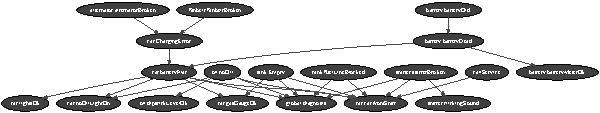
\includegraphics[width=\textwidth]{Figures/simpleCar2.pdf}
\caption{Réseau Bayésien utilisé pour tester les méthodes implémentées}
\label{FigReseauBayes}
\end{figure}

Dans les calculs de probabilités qu'il faut faire pour implémenter les algorithmes qui nous intéressent dans ce projet, les probabilités à calculer sont le plus souvent conditionnelles aux informations acquises. Afin de représenter les informations acquises et calcules les probabilités nécessaires de façon simple, nous utilisons la classe d'inférence exacte \texttt{LazyPropagation} de \texttt{pyAgrum}. Cette classe permet d'ajouter ou supprimer facilement des évidences au réseau Bayésien et obtenir facilement les lois de probabilité conditionnelles à ces évidences.

Cependant, la classe \texttt{LazyPropagation} ne permet pas de représenter les informations d'ordre \emph{temporelle}. En effet, assez souvent, les algorithmes demandent le calcul d'une probabilité de la forme «~quelle est la probabilité que le dispositif marche étant donné que l'on a fait telles et telles réparations et que le dispositif ne marchait pas avant~?~» Ce type de question demande de considérer l'état du dispositif à deux instants différents, alors qu'il n'est représenté que par un seul nœud dans le réseau Bayésien. Il faudrait dans ce cas utiliser des réseaux Bayésiens qui prennent en compte l'aspect temporel, ce qui est possible mais a pour conséquence d'augmenter la complexité à la fois d'implémentation et de calcul.

Afin de simplifier, nous utilisons alors une approximation proposée dans \cite{Heckerman_1995, heckerman1994troubleshooting}. Lorsque le dispositif n'a qu'une seule composante en panne (on parle alors de \emph{single fault assumption}), la probabilité que le dispositif marche suite à la réparation d'une composante $c_i$ est égale à la probabilité que cette composante était en panne avant sa réparation, soit
\[
P(o_0 = \text{normal} \mid c_i = \text{normal}, E) = P(c_i \neq \text{normal} \mid E).
\]
Selon \cite{Heckerman_1995, heckerman1994troubleshooting}, cette égalité, qui n'est plus valide sans la \emph{single fault assumption}, reste encore une bonne approximation pour la plupart de problèmes de \emph{Troubleshooting} d'intérêt, car il est rare en pratique qu'un dispositif tombe en panne à cause de plusieurs composantes simultanément fautives. Cette approximation a donc été utilisée dans toute l'implémentation présentée ici.

Outre le réseau Bayésien, la classe \texttt{TroubleShootingProblem} doit prendre en argument aussi les autres informations concernant le problème de \emph{Troubleshooting}~: quels nœuds du réseau Bayésien correspondent à des observations globales, à des composantes observables, à des composantes non-observables, au \emph{problem defining node} et à l'appel au service. En plus, il faut fournir également les coûts d'observation et de réparation nécessaires (ou les intervalles de coûts de réparation dans le cadre de la Section~\ref{SecContribElicitation}). Ces informations sont fournies par des dictionnaires passés en arguments lors de l'appel au constructeur de la classe \texttt{TroubleShootingProblem}.

La description de la Section~\ref{SecProbTrouble} demande aussi la donnée de l'état initial des informations, $E_0$. Lors de la création d'une instance de la classe \texttt{TroubleShootingProblem}, nous supposons que $E_0$ se réduit à la seule information que le dispositif ne marche pas à l'état initial. Il est possible de rajouter ou supprimer des informations manuellement à l'aide des méthodes \texttt{add\_evidence} et \texttt{remove\_evidence} avant d'appeler les algorithmes de résolution pour modifier le contenu de $E_0$.

\subsection{Algorithme simple}
\label{SecImplAlgoSimple}

Une première implémentation réalisée est celle de l'algorithme donné dans la Section~\ref{SecAlgoSimple}, qui a été codé dans la méthode \texttt{simple\_solver}. Cet algorithme polynomial résout le problème de \emph{Troubleshooting} de façon exacte sous les hypothèses simplificatrices de la Section~\ref{SecAlgoSimple} et peut être vu comme une première heuristique simple pour trouver une solution approchée de \eqref{MainProblem}. Seules les actions de réparation des composantes sont prises en compte. Comme rappelé dans une remarque dans la Section~\ref{SecArbresEtStrategies}, dans ce cadre simplifié une stratégie peut être vue comme une séquence d'actions. L'algorithme retourne alors cette séquence $S$, ainsi que l'espérance de coût $\EC(E_0, S)$.

\subsection{Algorithme simple avec observations locales}
\label{SecImplAlgoSimpleObs}

La deuxième implémentation réalisée est celle décrite au début de la Section~\ref{SecMyope}, qui correspond à une amélioration de l'algorithme simple et a été codée dans la méthode \texttt{simple\_solver\_\allowbreak{}obs}. Elle suppose que les seules actions possibles sont la réparation de composantes non-ob\-ser\-vables ou la paire observation-réparation des composantes observables. Comme pour l'implémentation précédente, une stratégie se réduit à une séquence d'actions et l'algorithme retourne la séquence calculée $S$ et l'espérance de coût correspondante $\EC(E_0, S)$.

\subsection{Algorithme myope}
\label{SecImplMyope}

L'algorithme myope décrit dans la Section~\ref{SecMyope} a été codé dans la méthode \texttt{myopic\_solver}. Par rapport aux deux algorithmes simples, l'algorithme myope rajoute la possibilité de réaliser des observations globales. Dans ce cas, la stratégie calculée $S$ n'est plus une simple séquence d'actions, car, à chaque fois qu'une observation est réalisée, la suite de l'algorithme dépend du résultat de cette observation et ne peut donc pas être connue au préalable.

On a ainsi fait le choix d'implémenter \texttt{myopic\_solver} de façon à faire \emph{un pas} de la résolution du problème de \emph{Troubleshooting} à chaque appel. L'idée est ainsi qu'un utilisateur doit faire appel à \texttt{myopic\_solver} pour savoir quelle est la prochaine action recommandée, cependant, l'action n'est pas réalisée~: c'est à l'utilisateur de la faire (ou décider d'en faire une autre s'il le souhaite) à travers les autres méthodes fournies et ensuite appeler à nouveau la fonction s'il souhaite connaître le prochain pas à réaliser. Une interface interactive en mode texte a été implémentée dans la méthode \texttt{myopic\_wraper}.

Une subtilité de \texttt{myopic\_solver} est qu'il faut parfois remettre en cause les résultats des observations. Si une observation a été réalisée et ensuite on réalise une réparation d'une composante qui peut affecter le résultat de cette observation, le résultat précédent n'est plus valide et il faut l'effacer. On a ainsi codé une méthode \texttt{observation\_obsolete} qui, étant donné un nœud qui vient d'être réparé, calcule tous les nœuds d'observation qui sont impactés par cette réparation. Cette fonction est utilisée par \texttt{myopic\_wraper} (et par l'interface graphique décrite dans la Section~\ref{SecImplInterface}) pour effacer ainsi les informations d'observations devenues obsolètes suite à une réparation.

La fonction \texttt{myopic\_solver} calcule, dans un premier temps, le coût espéré de réparation $\ECR$ sans la réalisation d'observations globales à l'aide de la méthode \texttt{simple\_solver\_obs}. Ensuite, pour chaque observation globale possible, la méthode calcule la valeur du coût espéré de réparation $\ECO$ si on réalise cette observation et puis applique \texttt{simple\_solver\_obs} pour trouver la suite des actions. La méthode choisit alors, parmi l'action proposée par le premier appel de \texttt{simple\_solver\_obs} et les observations globales, celle de plus petite espérance de coût.

Un autre point de vue possible et très similaire à l'approche myope est de considérer que, plutôt que de comparer chaque observation globale avec l'action retournée par \texttt{simple\_solver\_obs}, on peut comparer \emph{toutes} les actions possibles entre elles. Pour chaque action, on l'effectue et on utilise \texttt{simple\_solver\_obs} pour avoir une estimée du coût de réparation du reste de la séquence, et on choisit comme prochaine action à réaliser celle qui donne la plus petite valeur de coût espéré. L'avantage de cette méthode est de donner, à chaque action, une valeur d'espérance de coût, qui est celle estimée si l'action correspondante est la prochaine action à être prise. Cette modification de l'algorithme myope a été implémentée dans la méthode \texttt{ECR\_ECO\_wrapper}, qui retourne la meilleure action, son type, et les espérances de coût de toutes les autres actions possibles.

\subsection{Algorithme myope avec élicitation des coûts}
\label{SecImplElicitation}

Après avoir implémenté les trois algorithmes classiques de la Section~\ref{SecMethodesClassiques}, nous avons commencé l'implémentation des algorithmes décrits dans la Section~\ref{SecContribution} par celui de la Section~\ref{SecContribElicitation}, qui utilise l'élicitation pour améliorer les calculs quand on ne connaît pas la valeur exacte des coûts de réparation de quelques composantes. Puisque l'idée est de l'utiliser avec la méthode \texttt{myopic\_solver} (ou \texttt{ECR\_ECO\_solver}), les méthodes \texttt{best\_EVOI} et \texttt{elicitation} implémentées font uniquement la partie d'élicitation.

Notre implémentation permet à l'utilisateur de choisir à quel moment il veut répondre à des questions sur les coûts. Lorsque l'utilisateur le choisit, la méthode \texttt{best\_EVOI} doit être appelée. Cette méthode calcule les $\EVOI(E, c_i, \alpha)$ pour tous les composantes encore réparables $c_i$ et choisit celle de plus grande valeur. Comme indiqué dans la Section~\ref{SecContribElicitation}, le calcul des $\EVOI$ par la formule exacte \eqref{EqDefiEVOI} n'est pas souhaitable en pratique car cette formule fait intervenir la résolution exacte du problème de \emph{Troubleshooting}. On remplace ainsi le calcul exact des stratégies $S^\ast$, $S_-^\ast$ et $S_+^\ast$ de \eqref{EqSAsts} et des $\EC$ correspondants par un calcul approché en utilisant la méthode \texttt{simple\_solver\_obs}.

Une fois la meilleure question trouvée, la méthode \texttt{elicitation} permet de mettre à jour les informations sur les coûts à partir de la réponse de l'utilisateur. On remarque que \texttt{best\_EVOI} retourne toujours une question, même si celle-ci n'est pas intéressante à poser ($\EVOI$ égale à ou très proche de $0$). La gestion du choix de ne pas poser une question dans ce cas est fait directement par l'interface graphique dans notre implémentation.

\subsection{Algorithme exact}
\label{SecImplExact}

\textcolor{red}{TODO~!}

\subsection{Calcul de l'espérance de coût par une méthode de Monte-Carlo}
\label{SecImplMC}

Suivant les idées présentées dans la Section~\ref{SecCalculMonteCarlo}, nous avons implémenté plusieurs méthodes permettant d'approcher $\EC(E_0, S)$ pour les stratégies $S$ obtenues avec les algorithmes décrits dans les Sections~\ref{SecImplAlgoSimple} à \ref{SecImplExact}. Ces méthodes permettent aussi d'obtenir des statistiques sur le déroulement de la résolution du problème de \emph{Troubleshooting} avec les stratégies $S$. Elles ont toutes le suffixe \texttt{\_tester} dans leur nom.

Un de leurs arguments est \texttt{true\_prices}, un dictionnaire contenant les prix réels de réparation de chaque composante. En effet, un des intérêts de ces méthodes est de tester les algorithmes dans le cas où les prix réels de réparation des composantes ne sont pas connus et on applique les algorithmes soit avec les espérances de prix de réparation, soit en faisant des questions d'élicitation pour réduire l'incertitude sur ces prix. Ainsi, la séquence $S$ est toujours calculée avec les espérances de prix de réparation de chaque composante ou avec l'élicitation, mais la valeur du prix total de réparation retourné par les algorithmes \texttt{\_tester} est calculée en utilisant \texttt{true\_prices}.

Les autres arguments communs des méthodes \texttt{\_tester} sont la valeur de $\varepsilon$ à être utilisée pour le critère d'arrêt \eqref{EqCritereArret} et le nombres minimal et maximal d'itérations à être réalisées, \texttt{nb\_min} et \texttt{nb\_max}. Remarquons que \texttt{nb\_min} se fait nécessaire car l'algorithme peut trouver au début quelques fois de suite la même valeur de coût de réparation, auquel cas $s_n = 0$ et le critère d'arrêt \eqref{EqCritereArret} est satisfait, alors qu'on n'est pas encore à la convergence.

Les méthodes \texttt{\_tester} retournent toujours un booléen indiquant si l'algorithme s'est terminé après avoir atteint \texttt{nb\_max} itérations (cas \texttt{False}) ou à cause du critère d'arrêt \eqref{EqCritereArret} (cas \texttt{True}). Il retourne aussi les coûts trouvés, le nombre de réparations faites et, le cas échéant, le nombre d'observations globales faites ou de questions d'élicitation posées.

\subsection{Interface graphique}
\label{SecImplInterface}

L'interface graphique a été implémentée en utilisant le module \texttt{PyQt5}. Elle permet de sélectionner un des algorithmes décrits dans les Sections~\ref{SecImplAlgoSimple} à \ref{SecImplExact} et de l'utiliser pour résoudre le problème de \emph{Troubleshooting} dans le réseau présenté à la Section~\ref{SecImplRepresentation}. Alors que la sélection des algorithmes des Sections~\ref{SecImplAlgoSimple} et \ref{SecImplAlgoSimpleObs} donne juste la séquence d'actions à réaliser, les autres algorithmes utilisent un mode interactif qui, à chaque pas, donne l'action recommandée. Les algorithmes myopes (avec ou sans élicitation) permettent à l'utilisateur de choisir une autre action, alors que l'algorithme exact oblige le choix de l'action optimale donnée, mais ils attendent tous de l'utilisateur qu'il fournisse le résultat des actions. Un manuel d'utilisateur donne des explications détaillées de son utilisation et est fourni avec le code.

\section{Résultats}
\label{SecResultats}

% La propriété démontrée ci-dessus fait l'hypothèse cruciale que les valeurs de $\EC$ sont exactes. Or, l'algorithme que l'on utilise, basée sur l'idée de \cite{heckerman1994troubleshooting, Heckerman_1995}, est un algorithme heuristique glouton qui, malgré ses bons résultats pratiques, ne donne pas toujours la séquence de réparation avec le plus petit coût espéré, même si cela est souvent le cas. Ainsi, il se peut que l'on puisse trouver des valeurs négatives dans le calcul des $\EVOI$. En pratique, en testant avec des valeurs aléatoires pour les intervalles des coûts $[C_{\min}(r_i), C_{\max}(r_i)]$, on a observé des valeurs négatives pour $\EVOI$ dans $6\%$ des cas, mais cette valeur négative restait toujours petite, de l'ordre au maximum de $10^{-2}$, ce qui illustre d'ailleurs que l'algorithme de \cite{heckerman1994troubleshooting, Heckerman_1995} donne une bonne approximation.

% Il reste encore la question de quel $\alpha$ choisir pour chaque composante. Notre implémentation choisit toujours $\alpha = \overline C(r_i)$ pour la question correspondante à la composante $c_i$, ce qui est un choix raisonnable en absence d'autres informations car $\overline C(r_i)$ est l'espérance de la loi uniforme que l'on considère pour le coût $C(r_i)$. L'amélioration de ce choix naïf est une question intéressante qui pourrait permettre de poser des questions plus pertinentes à l'utilisateur. Pour espérer d'améliorer ce choix, il faut avoir plus d'information, ce que l'on pourrait obtenir, par exemple, en regardant ce que l'utilisateur choisit de faire lorsqu'il ne suit pas les recommandations du logiciel. En effet, dans ce cas, le fait que l'utilisateur n'a pas suivi une recommandation du logiciel indique qu'il a une connaissance en plus sur les valeurs de coût, ce que lui a fait de choisir une autre action. L'idée serait alors d'exploiter cette connaissance afin de modifier la loi de probabilité des coûts $C(r_i)$.

\bibliographystyle{abbrv}
\bibliography{bibliographie}

\end{document}
